\mainmatter

{\centering
	\chapter{Foundation}\label{parte1}
}

\thispagestyle{empty}
\noindent
\begin{minipage}[t]{0.35\textwidth}
	\begin{flushright}
		\large
		合抱之木，\\
		生於毫末；\\[0.5em]
		九層之臺，\\
		起於累土；\\[0.5em]
		千里之行，\\
		始於足下。
	\end{flushright}
\end{minipage}%
\hfill
\vrule
\hfill
\begin{minipage}[t]{0.48\textwidth}
	\raggedright
	\emph{
		$\!\!$A tree as big as a man's embrace\\
		grows from a tiny shoot;\\[0.5em]
		A tower of nine storeys\\
		begins with a heap of earth;\\[0.5em]
		The journey of a thousand Ii\\
		starts from where one stands. 
	}
\end{minipage}

\vspace{1em}
\hfill { 道德經 — \textsc{Dàodé jīng, Chapter 64}}

\section{围棋—Wéi Qí—, history and rules}
\setcounter{page}{1}

\subsection{History of Go in China}
The term 围棋 (Wéi Qí) originates from the characters 围 (Wéi), meaning ‘to surround,’ and 棋 (Qí), which refers to a ‘board game.’ In the West, it is commonly known as Go, a name derived from the Japanese 囲碁 (Igo). Although its exact chronology remains uncertain, ancient literary, pictorial, and archaeological records demonstrate that the game was an integral part of Chinese culture.
\begin{figure}[H]
	\centering
	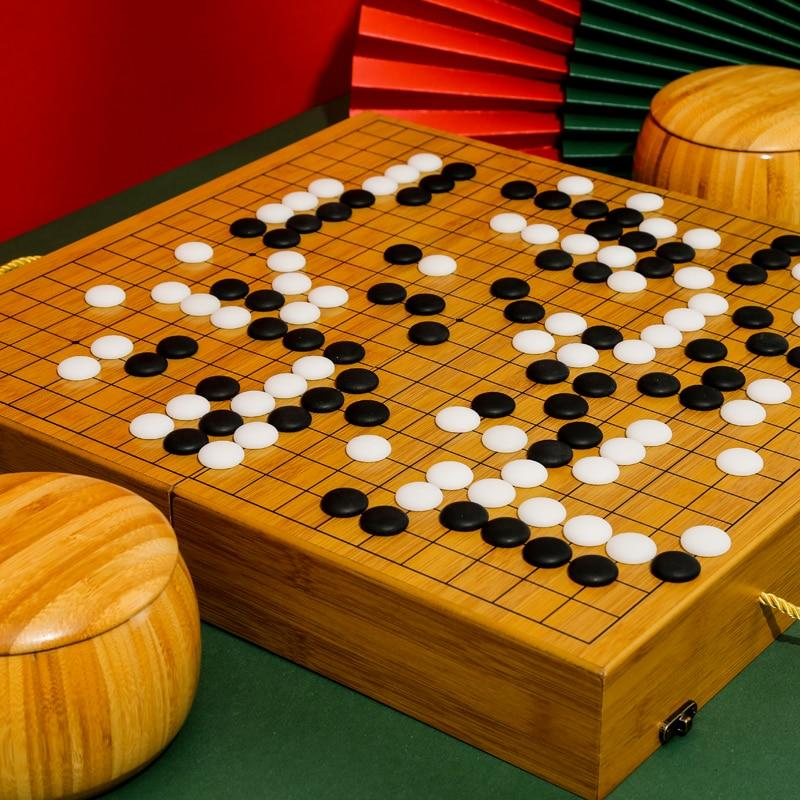
\includegraphics[width=0.51\linewidth]{figures/Go_1200x1200}
	\caption{A game of Go on a traditional board.}
	\label{fig:go1200x1200}
\end{figure}

Regarding its origins, mythical tradition holds that the legendary Emperor Yáo (堯) (2356–2257 BCE) invented it to enlighten the mind of his son, Dān Zhū (丹朱). Another account claims that Emperor Shùn (舜) (2255–2208 BCE) created it to educate his son, Shāng Jūn (商均). Furthermore, several sources attribute its invention to Wǔ, a vassal of Emperor Xià Jié (夏桀) (1818–1767 BCE), a courtier also celebrated for having devised the card game \cite{Smith}.

Sobre su origen, la tradición mítica afirma que el legendario emperador Yáo (堯) (2356-2257 a. e. c.) lo inventó con el propósito de iluminar la mente de su hijo, Dān Zhū (丹朱). Otra versión sostiene que fue el emperador Shùn (舜) (2255-2208 a. e. c.) quien lo creó para educar a su hijo, Shāng Jūn (商均). Asimismo, diversas fuentes atribuyen su invención a Wǔ, un vasallo del emperador Xià Jié (夏桀) (1818-1767 a. e. c.), cortesano célebre, además, por haber ideado el juego de cartas \cite{Smith}.

The first reliable mention of the game dates to the 3rd century BCE, when Mèngzǐ (孟軻) describes Yì Qiū (弈秋), a master of the game during the Warring States period who was recognized as one of the foremost exponents of his time. On the other hand, a notable game is preserved in the Wàngyōu Qīnglè Jí (忘憂清樂集), a mid-12th-century compilation. This work records one of the earliest recorded games, dating from the Han period (2nd century BCE – 2nd century CE) and contested between General Sūn Cè (孙策) and his captain Lǚ Fàn (Figure~\ref{fig:Fig 1}) \cite{Hist}. In conclusion, while it is unlikely that Go is 4,000 years old—as certain traditions suggest—its existence has been documented for at least 2,500 years. Its recurring appearance in texts and chronicles of the period suggests that, by then, the game enjoyed widespread enough familiarity for analogies based on it to be readily understood.
\begin{figure}
	\centering
	\begin{tikzpicture}[scale=0.45]
		\tikzstyle{every node}=[font=\small]
		% 1. DIBUJAR EL TABLERO
		\fill[goban] (-1.5,-1.5) rectangle (19.5,19.5);
		\draw[step=1cm, black] (0,0) grid (18,18);
		\draw[very thick] (0,0) rectangle (18,18);
		
		% 2. COORDENADAS
		\foreach \y [count=\i] in {0,...,18} {
			\node[black] at (-0.85, \y) {\i};
			\node[black] at (18.85, \y) {\i};
		}
		\foreach \x [count=\i] in {0,...,18} {
			\node[black] at (\x, -0.85) {\i};
			\node[black] at (\x, 18.85) {\i};
		}
		
		% Draw the central black dot
		\filldraw[black] (3,3) circle (4pt);
		\filldraw[black] (9,3) circle (4pt);
		\filldraw[black] (15,3) circle (4pt);
		
		\filldraw[black] (3,9) circle (4pt);
		\filldraw[black] (9,9) circle (4pt);
		\filldraw[black] (15,9) circle (4pt);
		
		\filldraw[black] (3,15) circle (4pt);
		\filldraw[black] (9,15) circle (4pt);
		\filldraw[black] (15,15) circle (4pt);
		
		\filldraw[black] (15,15) circle (13pt);
		\filldraw[black] (3,3) circle (13pt);
		\filldraw[draw=black,fill=white] (3,15) circle (13pt);
		\filldraw[draw=black,fill=white] (15,3) circle (13pt);
		
		\filldraw[draw=black,fill=white] (16,13) circle (13pt) node [color=black]{1};
		\filldraw[black] (12,16) circle (13pt) node [color=white]{2};
		\filldraw[draw=black,fill=white] (14,13) circle (13pt) node [color=black]{3};
		\filldraw[black] (16,8) circle (13pt) node [color=white]{4};
		\filldraw[draw=black,fill=white] (16,10) circle (13pt) node [color=black]{5};
		\filldraw[black] (16,5) circle (13pt) node [color=white]{6};
		\filldraw[draw=black,fill=white] (16,4) circle (13pt) node [color=black]{7};
		\filldraw[black] (15,5) circle (13pt) node [color=white]{8};
		\filldraw[draw=black,fill=white] (12,2) circle (13pt) node [color=black]{9};
		\filldraw[black] (10,2) circle (13pt) node [color=white]{10};
		\filldraw[draw=black,fill=white] (10,16) circle (13pt) node [color=black]{11};
		\filldraw[black] (17,14) circle (13pt) node [color=white]{12};
		\filldraw[draw=black,fill=white] (17,13) circle (13pt) node [color=black]{13};
		\filldraw[black] (7,2) circle (13pt) node [color=white]{14};
		\filldraw[draw=black,fill=white] (2,5) circle (13pt) node [color=black]{15};
		\filldraw[black] (2,10) circle (13pt) node [color=white]{16};
		\filldraw[draw=black,fill=white] (2,8) circle (13pt) node [color=black]{17};
		\filldraw[black] (2,13) circle (13pt) node [color=white]{18};
		\filldraw[draw=black,fill=white] (5,2) circle (13pt) node [color=black]{19};
		\filldraw[black] (5,3) circle (13pt) node [color=white]{20};
		\filldraw[draw=black,fill=white] (2,2) circle (13pt) node [color=black]{21};
		\filldraw[black] (3,2) circle (13pt) node [color=white]{22};
		\filldraw[draw=black,fill=white] (2,3) circle (13pt) node [color=black]{23};
		\filldraw[black] (2,1) circle (13pt) node [color=white]{24};
		\filldraw[draw=black,fill=white] (1,1) circle (13pt) node [color=black]{25};
		\filldraw[black] (3,1) circle (13pt) node [color=white]{26};
		\filldraw[draw=black,fill=white] (2,14) circle (13pt) node [color=black]{27};
		\filldraw[black] (3,13) circle (13pt) node [color=white]{28};
		\filldraw[draw=black,fill=white] (6,16) circle (13pt) node [color=black]{29};
		\filldraw[black] (16,2) circle (13pt) node [color=white]{30};
		\filldraw[draw=black,fill=white] (15,2) circle (13pt) node [color=black]{31};
		\filldraw[black] (17,4) circle (13pt) node [color=white]{32};
		\filldraw[draw=black,fill=white] (17,3) circle (13pt) node [color=black]{33};
		\filldraw[black] (16,4) circle (13pt) node [color=white]{34};
		\filldraw[draw=black,fill=white] (17,3) circle (13pt) node [color=black]{35};
		\filldraw[black] (14,6) circle (13pt) node [color=white]{36};
		\filldraw[draw=black,fill=white] (16,1) circle (13pt) node [color=black]{37};
		\filldraw[black] (1,7) circle (13pt) node [color=white]{38};
		\filldraw[draw=black,fill=white] (12,6) circle (13pt) node [color=black]{39};
		\filldraw[black] (1,8) circle (13pt) node [color=white]{40};
		\filldraw[draw=black,fill=white] (11,14) circle (13pt) node [color=black]{41};
		\filldraw[black] (14,16) circle (13pt) node [color=white]{42};
		\filldraw[draw=black,fill=white] (5,14) circle (13pt) node [color=black]{43};
	\end{tikzpicture}
	\caption{
		Game between \textit{Sūn Cè} and \textit{Lǚ Fàn}. The unnumbered stones are due to the fact that, at that time, games began from a predetermined starting position and White played first.}
	\label{fig:Fig 1}
\end{figure}

\subsection{Historia del Go en la Argentina}

\subsection{History of Go in Argentina}

Engineer Hilario Fernández Long was the pioneer of Go in Argentina. After learning the fundamentals from a Japanese friend, his enthusiasm led him to teach the first courses on the discipline at the Centro Argentino de Ingenieros (Argentine Center of Engineers). Thanks to his efforts, the Asociación Argentina de Go (Argentine Go Association) was founded on September 11, 1971. Later, in 1974, Fernández Long published the \textit{Manual de Go} alongside Adalberto Moderc, which was followed in 1983 by the work \textit{Introducción al Go} \cite{Long83}.  

It is imperative to highlight the figure of Fernando Aguilar \cite{Long_Hubert, Aguilar2, Aguilar1}, Fernández Long's first cousin once removed and arguably the foremost exponent of Go in argentina. Although he took his first steps in the world of strategy games through chess, under the tutelage of his father, Pedro Antonio Aguilar, Fernando discovered Go through the print media\footnote{I'll translate his words but preserve the original.}:

\begin{quote}
	«En mi casa se compraba el diario \textit{La Nación}. Allí se publicaban periódicamente notas de ajedrez […] En cierto momento empezaron a aparecer notas sobre Go. El autor era el mismo que publicaba las de ajedrez».
	
	``At home, we used to buy the newspaper \textit{La Nación}. Chess columns were published there regularly [\dots] At a certain point, articles about Go began to appear. The author was the same person who wrote the chess ones.''
\end{quote}
Driven by curiosity, he consulted his father, who replied:
\begin{quote}
	«Vayamos a visitar a tu tío Hilario para que nos enseñe a jugar al Go».
	
	``Let's go visit your uncle Hilario so he can teach us how to play Go.''
\end{quote}
Aguilar, at the age of twelve~\cite{Aguilar3}, recalls his beginnings as follows:
\begin{quote}
	«Hilario nos explicó las reglas, nos dio algunas líneas generales. En la despedida nos regaló un juego de tablero y piedras y un libro, el ​\textit{How to play Go}, una versión en inglés de un libro de \textit{Takagawa Shukaku} [...] A partir de ahí, las sesiones de estudio con mi padre consistieron en la lectura de un capítulo del libro que él me traducía del inglés, seguida de una partida que jugábamos entre nosotros».
	
	``Hilario explained the rules to us and gave us some general guidelines. As we parted, he gave us a board and stones set, as well as a book: \textit{How to Play Go}, an English translation of a work by \textit{Takagawa Shukaku} [\dots] From then on, the study sessions with my father consisted of reading a chapter of the book—which he translated for me from English—followed by a game played between us.''
\end{quote}
Having mastered the rules, it was time to compete.
\begin{quote}
	«Corría el año 1972 y la actividad de Go en el país estaba en plena efervescencia. En septiembre de ese año visitó nuestro país el maestro \textit{Iwamoto Kaoru}.»
	
	``The year was 1972, and Go activity across the country was in full swing. In September of that year, Master \textit{Iwamoto Kaoru} visited our country.''
\end{quote}
Following the match between \textit{Enrique Lindenbaum} and \textit{Iwamoto}, it was the amateurs' turn:
\begin{quote}
	«Luego vino la sesión de simultáneas, donde tuve la primera experiencia de enfrentar a una jugadora profesional. Yo tenía nivel de principiante (o poco más) y debía poner 9 piedras, pero \textit{Sachiko Kondo} pidió jugar con 7 piedras [...] Cuando quedó claro que la victoria de Blanco era aplastante, la profesional pidió suspender el juego».
	
	``Then came the simultaneous exhibition, where I had my first experience facing a professional player. I was at a beginner's level (or slightly above) and was supposed to take a nine-stone handicap, but \textit{Sachiko Kondo} asked to play with seven stones [\dots] When it became evident that White's victory was overwhelming, the professional asked to suspend the game.''\footnote{Since Aguilar was the weaker player, he played first (taking Black), leaving \textit{Kondo} to play with White.}
\end{quote}
Despite the defeat, \textit{Fernando's} ambition only continued to grow:
\begin{quote}
	«El paso siguiente que dimos con mi padre fue hacernos socios de la Asociación Argentina de Go […] Pronto vino el torneo por la ​\textit{Copa La Nación}. En 1972 se jugó la segunda edición».
	
	``The next step my father and I took was joining the Argentine Go Association [\dots] Soon after came the \textit{Copa La Nación} tournament. Its second edition took place in 1972.''
\end{quote}
Although he did not have a standout performance that year, he certainly did the following year:
\begin{quote}
	«Ya entrado el año 1973, llegó el momento de disputar la tercera edición de la \textit{Copa La Nación} […] El torneo fue muy disputado, pero pude ganarlo invicto, relegando al segundo lugar a \textit{Pedro Hecht}».
	
	``Well into 1973, the time came to contest the third edition of the \textit{Copa La Nación} [\dots] The tournament was fiercely contested, but I managed to win it undefeated, relegating \textit{Pedro Hecht} to second place.''
\end{quote}
The most significant milestone of his career came in 2002. After securing third place in the \textit{Ibero-American Cup}, he qualified for the 1st \textit{Toyota \& Denso Cup -- World Go Oza}. In the first round, on March 19, he faced \textit{Hasegawa Sunao} ($9p$) (Figure~\ref{fig:aguilar_hasegawa_1}). The opening proceeded customarily:
\begin{quote}
	«Tomé una cantidad abundante de piedras y mi adversario adivinó correctamente que se trataba de un número impar, así que le correspondió jugar con negras».
	
	``I grabbed a handful of stones, and my opponent guessed correctly that it was an odd number, so he was assigned to play with Black.''\footnote{To determine who plays first, Japanese tradition employs a method called \textit{Nigiri} (握り). The senior or higher-ranked player takes a handful of white stones and conceals them in hand. The opponent then places one black stone on the board to guess an odd count, or two black stones to guess an even count. Next, the white stones are counted in pairs; if the opponent guesses correctly, they play with the black stones and make the first move. If mistaken, they play with White.}
\end{quote}
Against all odds, the game ended in \textit{Aguilar's} favor:
\begin{quote}
	«La diferencia final fue de 3,5 puntos a mi favor. A mí me llamó la atención el margen y a Hasegawa lo sorprendió: pidió la copia del partido y estuvo un rato largo confirmando que era efectivamente así».
	
	``The final margin was 3.5 points in my favor. The difference caught my attention, and it surprised Hasegawa: he asked for the game record and spent quite a while confirming that it was indeed so.''
\end{quote}
\begin{figure}[H]
	\centering
	\begin{tikzpicture}[scale=0.45]
		\tikzstyle{every node}=[font=\small]
		% --- ESTILOS DE LAS PIEDRAS ---
		% Piedra Negra: fondo negro, texto blanco
		\tikzstyle{black stone}=[draw=black, fill=black, circle, minimum size=13pt, inner sep=0pt, text=white, ]
		% Piedra Blanca: fondo blanco, borde negro, texto negro
		\tikzstyle{white stone}=[draw=black, fill=white, circle, minimum size=13pt, inner sep=0pt, text=black,]
		%font=\bfseries\tiny
		% 1. DIBUJAR EL TABLERO
		% Fondo
		\fill[goban] (-1.5,-1.5) rectangle (19.5,19.5);
		
		% Grilla
		\draw[step=1cm, black] (0,0) grid (18,18);
		
		% Borde grueso
		\draw[very thick] (0,0) rectangle (18,18);
		
		% 2. COORDENADAS (Optimizado con bucles)
		% Eje Y (Números 1-19) - Nota: TikZ 0 es la fila 1 visual
		\foreach \y [count=\i] in {0,...,18} {
			\node[black] at (-0.85, \y) {\i};
			\node[black] at (18.85, \y) {\i};
		}
		% Eje X (Números 1-19)
		\foreach \x [count=\i] in {0,...,18} {
			\node[black] at (\x, -0.85) {\i};
			\node[black] at (\x, 18.85) {\i};
		}
		
		% 3. HOSHI (Puntos estelares)
		\foreach \x in {3,9,15} {
			\foreach \y in {3,9,15} {
				\filldraw[black] (\x,\y) circle (3pt);
			}
		}
		\filldraw[black] (16,15) circle (12pt) ; % B[qd]
		\filldraw[black] (4,2) circle (12pt) ;   % B[eq]
		\filldraw[black] (2,14) circle (12pt) ;  % B[ce]
		\filldraw[black] (7,16) circle (12pt) ;  % B[hc]
		\filldraw[black] (4,14) circle (12pt) ;  % B[ee]
		\filldraw[black] (3,15) circle (12pt) ;  % B[dd]
		\filldraw[black] (4,16) circle (12pt) ;  % B[ec]
		\filldraw[black] (5,16) circle (12pt) ;  % B[fc]
		\filldraw[black] (1,13) circle (12pt) ;  % B[bf]
		\filldraw[black] (2,13) circle (12pt) ;  % B[cf]
		\filldraw[black] (17,3) circle (12pt) ;  % B[rp]
		\filldraw[black] (16,14) circle (12pt) ; % B[qe]
		\filldraw[black] (15,16) circle (12pt) ; % B[pc]
		\filldraw[black] (16,12) circle (12pt) ; % B[qg]
		\filldraw[black] (14,5) circle (12pt) ;  % B[on]
		\filldraw[black] (10,2) circle (12pt) ;  % B[kq]
		\filldraw[black] (10,4) circle (12pt) ;  % B[ko]
		\filldraw[black] (10,6) circle (12pt) ;  % B[km]
		\filldraw[black] (15,12) circle (12pt) ; % B[pg]
		\filldraw[black] (16,13) circle (12pt) ; % B[qf]
		\filldraw[black] (14,15) circle (12pt) ; % B[od]
		\filldraw[black] (15,17) circle (12pt) ; % B[pb]
		\filldraw[black] (7,3) circle (12pt) ;   % B[hp]
		\filldraw[black] (2,5) circle (12pt) ;   % B[cn]
		\filldraw[black] (5,6) circle (12pt) ;   % B[fm]
		\filldraw[black] (5,7) circle (12pt) ;   % B[fl]
		\filldraw[black] (8,7) circle (12pt) ;   % B[il]
		\filldraw[black] (8,8) circle (12pt) ;   % B[ik]
		\filldraw[black] (5,3) circle (12pt) ;   % B[fp]
		\filldraw[black] (6,3) circle (12pt) ;   % B[gp]
		\filldraw[black] (7,2) circle (12pt) ;   % B[hq]
		\filldraw[black] (8,1) circle (12pt) ;   % B[ir]
		\filldraw[black] (9,1) circle (12pt) ;   % B[jr]
		\filldraw[black] (4,3) circle (12pt) ;   % B[ep]
		\filldraw[black] (3,4) circle (12pt) ;   % B[do]
		\filldraw[black] (7,8) circle (12pt) ;   % B[hk]
		\filldraw[black] (3,5) circle (12pt) ;   % B[dn]
		\filldraw[black] (15,15) circle (12pt) ; % B[pd]
		\filldraw[black] (10,12) circle (12pt) ; % B[kg]
		%\filldraw[black] (5,9) circle (12pt) ;   % B[fk]
		\filldraw[black] (12,12) circle (12pt) ; % B[mg]
		\filldraw[black] (12,11) circle (12pt) ; % B[mh]
		\filldraw[black] (13,10) circle (12pt) ; % B[ni]
		\filldraw[black] (13,11) circle (12pt) ; % B[nh]
		\filldraw[black] (12,9) circle (12pt) ;  % B[mj]
		\filldraw[black] (11,10) circle (12pt) ; % B[li]
		\filldraw[black] (13,7) circle (12pt) ;  % B[nl]
		\filldraw[black] (13,8) circle (12pt) ;  % B[nk]
		\filldraw[black] (12,3) circle (12pt) ;  % B[mp]
		\filldraw[black] (13,4) circle (12pt) ;  % B[no]
		\filldraw[black] (12,2) circle (12pt) ;  % B[mq]
		\filldraw[black] (13,5) circle (12pt) ;  % B[nn]
		\filldraw[black] (15,6) circle (12pt) ;  % B[pm]
		\filldraw[black] (14,6) circle (12pt) ;  % B[om]
		\filldraw[black] (14,8) circle (12pt) ;  % B[ok]
		\filldraw[black] (15,9) circle (12pt) ;  % B[pj]
		\filldraw[black] (14,10) circle (12pt) ; % B[oi]
		\filldraw[black] (14,9) circle (12pt) ;  % B[oj]
		\filldraw[black] (4,9) circle (12pt) ;   % B[ej]
		\filldraw[black] (4,10) circle (12pt) ;  % B[ei]
		\filldraw[black] (17,14) circle (12pt) ; % B[re]
		\filldraw[black] (18,15) circle (12pt) ; % B[sd]
		\filldraw[black] (8,11) circle (12pt) ;  % B[ih]
		\filldraw[black] (14,18) circle (12pt) ; % B[oa]
		\filldraw[black] (12,1) circle (12pt) ;  % B[mr]
		\filldraw[black] (7,12) circle (12pt) ;  % B[hg]
		\filldraw[black] (6,13) circle (12pt) ;  % B[gf]
		\filldraw[black] (5,14) circle (12pt) ;  % B[fe]
		\filldraw[black] (6,12) circle (12pt) ;  % B[gg]
		\filldraw[black] (7,14) circle (12pt) ;  % B[he]
		\filldraw[black] (10,13) circle (12pt) ; % B[kf]
		\filldraw[black] (12,13) circle (12pt) ; % B[mf]
		\filldraw[black] (11,14) circle (12pt) ; % B[le]
		\filldraw[black] (6,15) circle (12pt) ;  % B[gd]
		\filldraw[black] (6,16) circle (12pt) ;  % B[gc]
		\filldraw[black] (13,0) circle (12pt) ;  % B[ns]
		\filldraw[black] (12,0) circle (12pt) ;  % B[ms]
		\filldraw[black] (3,11) circle (12pt) ;  % B[dh]
		\filldraw[black] (4,5) circle (12pt) ;   % B[en]
		\filldraw[black] (17,17) circle (12pt) ; % B[rb]
		\filldraw[black] (2,6) circle (12pt) ;   % B[cm]
		\filldraw[black] (11,15) circle (12pt) ; % B[ld]
		\filldraw[black] (11,12) circle (12pt) ; % B[lg]
		\filldraw[black] (7,0) circle (12pt) ;   % B[hs]
		\filldraw[black] (8,0) circle (12pt) ;   % B[is]
		\filldraw[black] (15,18) circle (12pt) ; % B[pa]
		\filldraw[black] (0,13) circle (12pt) ;  % B[af]
		\filldraw[black] (9,11) circle (12pt) ;  % B[jh]
		\filldraw[black] (8,16) circle (12pt) ;  % B[ic]
		\filldraw[black] (0,14) circle (12pt) ;  % B[ae]
		\filldraw[black] (14,14) circle (12pt) ; % B[oe]
		\filldraw[black] (11,13) circle (12pt) ; % B[lf]
		\filldraw[black] (3,12) circle (12pt) ;  % B[dg]
		\filldraw[black] (3,10) circle (12pt) ;  % B[di]
		\filldraw[black] (3,6) circle (12pt) ;   % B[dm]
		\filldraw[black] (5,5) circle (12pt) ;   % B[fn]
		\filldraw[black] (5,8) circle (12pt) ;   % B[fn]
		\filldraw[black] (16,5) circle (12pt) ;   % B[fn]
		\filldraw[black] (16,8) circle (12pt) ;   % B[fn]
		
		% --- PIEDRAS BLANCAS (Fernando Aguilar) ---
		\filldraw[draw=black,fill=white] (15,3) circle (12pt) ;  % W[pp]
		\filldraw[draw=black,fill=white] (3,16) circle (12pt) ;  % W[dc]
		\filldraw[draw=black,fill=white] (14,16) circle (12pt) ; % W[oc]
		\filldraw[draw=black,fill=white] (2,10) circle (12pt) ;  % W[ci]
		\filldraw[draw=black,fill=white] (11,16) circle (12pt) ; % W[lc]
		\filldraw[draw=black,fill=white] (2,15) circle (12pt) ;  % W[cd]
		\filldraw[draw=black,fill=white] (1,16) circle (12pt) ;  % W[bc]
		\filldraw[draw=black,fill=white] (2,16) circle (12pt) ;  % W[cc]
		\filldraw[draw=black,fill=white] (4,17) circle (12pt) ;  % W[eb]
		\filldraw[draw=black,fill=white] (1,14) circle (12pt) ;  % W[be]
		\filldraw[draw=black,fill=white] (0,15) circle (12pt) ;  % W[ad]
		\filldraw[draw=black,fill=white] (2,7) circle (12pt) ;   % W[cl]
		\filldraw[draw=black,fill=white] (13,2) circle (12pt) ;  % W[nq]
		\filldraw[draw=black,fill=white] (16,2) circle (12pt) ;  % W[qq]
		\filldraw[draw=black,fill=white] (15,14) circle (12pt) ; % W[pe]
		\filldraw[draw=black,fill=white] (15,13) circle (12pt) ; % W[pf]
		\filldraw[draw=black,fill=white] (14,17) circle (12pt) ; % W[ob]
		\filldraw[draw=black,fill=white] (8,2) circle (12pt) ;   % W[iq]
		\filldraw[draw=black,fill=white] (14,11) circle (12pt) ; % W[oh]
		\filldraw[draw=black,fill=white] (8,4) circle (12pt) ;   % W[io]
		\filldraw[draw=black,fill=white] (17,2) circle (12pt) ;  % W[rq]
		\filldraw[draw=black,fill=white] (16,11) circle (12pt) ; % W[qh]
		\filldraw[draw=black,fill=white] (14,12) circle (12pt) ; % W[og]
		\filldraw[draw=black,fill=white] (15,11) circle (12pt) ; % W[ph]
		\filldraw[draw=black,fill=white] (13,14) circle (12pt) ; % W[ne]
		\filldraw[draw=black,fill=white] (13,15) circle (12pt) ; % W[nd]
		\filldraw[draw=black,fill=white] (8,3) circle (12pt) ;   % W[ip]
		\filldraw[draw=black,fill=white] (4,7) circle (12pt) ;   % W[el]
		\filldraw[draw=black,fill=white] (8,6) circle (12pt) ;   % W[im]
		\filldraw[draw=black,fill=white] (4,8) circle (12pt) ;   % W[ek]
		\filldraw[draw=black,fill=white] (7,7) circle (12pt) ;   % W[hl]
		\filldraw[draw=black,fill=white] (5,2) circle (12pt) ;   % W[fq]
		\filldraw[draw=black,fill=white] (6,2) circle (12pt) ;   % W[gq]
		\filldraw[draw=black,fill=white] (4,1) circle (12pt) ;   % W[er]
		\filldraw[draw=black,fill=white] (7,1) circle (12pt) ;   % W[hr]
		\filldraw[draw=black,fill=white] (6,1) circle (12pt) ;   % W[gr]
		\filldraw[draw=black,fill=white] (3,2) circle (12pt) ;   % W[dq]
		\filldraw[draw=black,fill=white] (3,3) circle (12pt) ;   % W[dp]
		\filldraw[draw=black,fill=white] (2,2) circle (12pt) ;   % W[cq]
		\filldraw[draw=black,fill=white] (1,3) circle (12pt) ;   % W[bp]
		\filldraw[draw=black,fill=white] (2,4) circle (12pt) ;   % W[co]
		\filldraw[draw=black,fill=white] (1,5) circle (12pt) ;   % W[bn]
		\filldraw[draw=black,fill=white] (0,5) circle (12pt) ;   % W[ao]
		\filldraw[draw=black,fill=white] (9,16) circle (12pt) ;  % W[jc]
		\filldraw[draw=black,fill=white] (9,14) circle (12pt) ;  % W[je]
		\filldraw[draw=black,fill=white] (11,11) circle (12pt) ; % W[lh]
		\filldraw[draw=black,fill=white] (15,7) circle (12pt) ;  % W[pl]
		\filldraw[draw=black,fill=white] (16,7) circle (12pt) ;  % W[ql]
		\filldraw[draw=black,fill=white] (14,7) circle (12pt) ;  % W[ol]
		\filldraw[draw=black,fill=white] (17,11) circle (12pt) ; % W[rh]
		\filldraw[draw=black,fill=white] (13,3) circle (12pt) ;  % W[np]
		\filldraw[draw=black,fill=white] (12,4) circle (12pt) ;  % W[mo]
		\filldraw[draw=black,fill=white] (14,4) circle (12pt) ;  % W[oo]
		\filldraw[draw=black,fill=white] (15,5) circle (12pt) ;  % W[pn]
		\filldraw[draw=black,fill=white] (15,4) circle (12pt) ;  % W[po]
		\filldraw[draw=black,fill=white] (16,6) circle (12pt) ;  % W[qm]
		\filldraw[draw=black,fill=white] (15,8) circle (12pt) ;  % W[pk]
		\filldraw[draw=black,fill=white] (16,9) circle (12pt) ;  % W[qj]
		\filldraw[draw=black,fill=white] (15,10) circle (12pt) ; % W[pi]
		\filldraw[draw=black,fill=white] (13,13) circle (12pt) ; % W[nf]
		\filldraw[draw=black,fill=white] (3,9) circle (12pt) ;   % W[dj]
		\filldraw[draw=black,fill=white] (18,14) circle (12pt) ; % W[se]
		\filldraw[draw=black,fill=white] (18,12) circle (12pt) ; % W[sg]
		\filldraw[draw=black,fill=white] (8,13) circle (12pt) ;  % W[if]
		\filldraw[draw=black,fill=white] (5,17) circle (12pt) ;  % W[fb]
		\filldraw[draw=black,fill=white] (12,17) circle (12pt) ; % W[mb]
		\filldraw[draw=black,fill=white] (13,1) circle (12pt) ;  % W[nr]
		\filldraw[draw=black,fill=white] (7,13) circle (12pt) ;  % W[hf]
		%\filldraw[draw=black,fill=white] (6,14) circle (12pt) ;  % W[ge]
		\filldraw[draw=black,fill=white] (8,12) circle (12pt) ;  % W[ig]
		\filldraw[draw=black,fill=white] (1,11) circle (12pt) ;  % W[bh]
		\filldraw[draw=black,fill=white] (10,14) circle (12pt) ; % W[ke]
		\filldraw[draw=black,fill=white] (6,17) circle (12pt) ;  % W[gb]
		\filldraw[draw=black,fill=white] (7,15) circle (12pt) ;  % W[hd]
		\filldraw[draw=black,fill=white] (8,15) circle (12pt) ;  % W[id]
		\filldraw[draw=black,fill=white] (7,17) circle (12pt) ;  % W[hb]
		\filldraw[draw=black,fill=white] (14,0) circle (12pt) ;  % W[os]
		\filldraw[draw=black,fill=white] (14,1) circle (12pt) ;  % W[or]
		\filldraw[draw=black,fill=white] (4,6) circle (12pt) ;   % W[em]
		\filldraw[draw=black,fill=white] (18,13) circle (12pt) ; % W[sf]
		\filldraw[draw=black,fill=white] (12,14) circle (12pt) ; % W[me]
		\filldraw[draw=black,fill=white] (1,6) circle (12pt) ;   % W[bm]
		\filldraw[draw=black,fill=white] (10,15) circle (12pt) ; % W[kd]
		\filldraw[draw=black,fill=white] (13,18) circle (12pt) ; % W[na]
		\filldraw[draw=black,fill=white] (6,0) circle (12pt) ;   % W[gs]
		\filldraw[draw=black,fill=white] (3,1) circle (12pt) ;   % W[dr]
		\filldraw[draw=black,fill=white] (2,11) circle (12pt) ;  % W[ch]
		\filldraw[draw=black,fill=white] (9,12) circle (12pt) ;  % W[jg]
		\filldraw[draw=black,fill=white] (12,15) circle (12pt) ; % W[md]
		\filldraw[draw=black,fill=white] (8,17) circle (12pt) ;  % W[ib]
		\filldraw[draw=black,fill=white] (1,15) circle (12pt) ;  % W[bd]
		\filldraw[draw=black,fill=white] (14,13) circle (12pt) ; % W[of]
		\filldraw[draw=black,fill=white] (2,12) circle (12pt) ;  % W[cg]
		\filldraw[draw=black,fill=white] (0,11) circle (12pt) ;  % W[ah]
		\filldraw[draw=black,fill=white] (2,8) circle (12pt) ;   % W[ck]
		\filldraw[draw=black,fill=white] (3,7) circle (12pt) ;   % W[dl]
		\filldraw[draw=black,fill=white] (17,12) circle (12pt) ; % W[rg]
		
		% --- TERRITORIOS BLANCOS (Fernando Aguilar - Blue) ---
		\filldraw[Blue] (0,0) circle (6pt);
		\filldraw[Blue] (1,0) circle (6pt);
		\filldraw[Blue] (2,0) circle (6pt);
		\filldraw[Blue] (3,0) circle (6pt);
		\filldraw[Blue] (4,0) circle (6pt);
		\filldraw[Blue] (5,0) circle (6pt);
		\filldraw[Blue] (0,1) circle (6pt);
		\filldraw[Blue] (1,1) circle (6pt);
		\filldraw[Blue] (2,1) circle (6pt);
		\filldraw[Blue] (5,1) circle (6pt);
		\filldraw[Blue] (0,2) circle (6pt);
		\filldraw[Blue] (1,2) circle (6pt);
		\filldraw[Blue] (0,3) circle (6pt);
		\filldraw[Blue] (0,4) circle (6pt);
		\filldraw[Blue] (0,6) circle (6pt);
		\filldraw[Blue] (0,7) circle (6pt);
		\filldraw[Blue] (1,7) circle (6pt);
		\filldraw[Blue] (0,8) circle (6pt);
		\filldraw[Blue] (1,8) circle (6pt);
		\filldraw[Blue] (0,9) circle (6pt);
		\filldraw[Blue] (1,9) circle (6pt);
		\filldraw[Blue] (0,10) circle (6pt);
		\filldraw[Blue] (1,10) circle (6pt);
		%	\filldraw[Blue] (0,11) circle (6pt);
		%	\filldraw[Blue] (1,11) circle (6pt);
		%		\filldraw[Blue] (0,12) circle (6pt);
		%	\filldraw[Blue] (1,12) circle (6pt);
		\filldraw[Blue] (9,15) circle (6pt);
		\filldraw[Blue] (9,17) circle (6pt);
		\filldraw[Blue] (10,17) circle (6pt);
		\filldraw[Blue] (10,16) circle (6pt);
		\filldraw[Blue] (11,17) circle (6pt);
		\filldraw[Blue] (13,17) circle (6pt);
		\filldraw[Blue] (13,16) circle (6pt);
		\filldraw[Blue] (12,16) circle (6pt);
		\filldraw[Blue] (2,9) circle (6pt);
		\filldraw[Blue] (3,8) circle (6pt);
		\filldraw[Blue] (1,4) circle (6pt);
		\filldraw[Blue] (2,3) circle (6pt);
		\filldraw[Blue] (0,16) circle (6pt);
		\filldraw[Blue] (0,17) circle (6pt);
		\filldraw[Blue] (1,17) circle (6pt);
		\filldraw[Blue] (2,17) circle (6pt);
		\filldraw[Blue] (3,17) circle (6pt);
		\filldraw[Blue] (0,18) circle (6pt);
		\filldraw[Blue] (1,18) circle (6pt);
		\filldraw[Blue] (2,18) circle (6pt);
		\filldraw[Blue] (3,18) circle (6pt);
		\filldraw[Blue] (4,18) circle (6pt);
		\filldraw[Blue] (5,18) circle (6pt);
		\filldraw[Blue] (6,18) circle (6pt);
		\filldraw[Blue] (7,18) circle (6pt);
		\filldraw[Blue] (8,18) circle (6pt);
		\filldraw[Blue] (9,18) circle (6pt);
		\filldraw[Blue] (10,18) circle (6pt);
		\filldraw[Blue] (11,18) circle (6pt);
		\filldraw[Blue] (12,18) circle (6pt);
		
		% Lado derecho (Territorio consolidado y capturas)
		\filldraw[Blue] (15,0) circle (6pt);
		\filldraw[Blue] (16,0) circle (6pt);
		\filldraw[Blue] (17,0) circle (6pt);
		\filldraw[Blue] (18,0) circle (6pt);
		\filldraw[Blue] (15,1) circle (6pt);
		\filldraw[Blue] (16,1) circle (6pt);
		\filldraw[Blue] (17,1) circle (6pt);
		\filldraw[Blue] (18,1) circle (6pt);
		\filldraw[Blue] (14,2) circle (6pt);
		\filldraw[Blue] (15,2) circle (6pt);
		\filldraw[Blue] (18,2) circle (6pt);
		\filldraw[Blue] (14,3) circle (6pt);
		\filldraw[Blue] (16,3) circle (6pt);
		\filldraw[Blue] (18,3) circle (6pt);
		\filldraw[Blue] (16,4) circle (6pt);
		\filldraw[Blue] (17,4) circle (6pt);
		\filldraw[Blue] (18,4) circle (6pt);
		\filldraw[Blue] (16,5) circle (6pt);
		\filldraw[Blue] (17,5) circle (6pt);
		\filldraw[Blue] (18,5) circle (6pt);
		\filldraw[Blue] (17,6) circle (6pt);
		\filldraw[Blue] (18,6) circle (6pt);
		\filldraw[Blue] (17,7) circle (6pt);
		\filldraw[Blue] (18,7) circle (6pt);
		\filldraw[Blue] (16,8) circle (6pt);
		\filldraw[Blue] (17,8) circle (6pt);
		\filldraw[Blue] (18,8) circle (6pt);
		\filldraw[Blue] (17,9) circle (6pt);
		\filldraw[Blue] (18,9) circle (6pt);
		\filldraw[Blue] (16,10) circle (6pt);
		\filldraw[Blue] (17,10) circle (6pt);
		\filldraw[Blue] (18,10) circle (6pt);
		\filldraw[Blue] (18,11) circle (6pt);
		\filldraw[Blue] (17,3) circle (6pt);
		
		% --- TERRITORIOS NEGROS (Hasegawa Sunao - OliveGreen) ---
		% Abajo centro
		\filldraw[OliveGreen] (9,0) circle (6pt);
		\filldraw[OliveGreen] (10,0) circle (6pt);
		\filldraw[OliveGreen] (11,0) circle (6pt);
		\filldraw[OliveGreen] (10,1) circle (6pt);
		\filldraw[OliveGreen] (11,1) circle (6pt);
		\filldraw[OliveGreen] (11,2) circle (6pt);
		\filldraw[OliveGreen] (11,3) circle (6pt);
		\filldraw[OliveGreen] (11,4) circle (6pt);
		\filldraw[OliveGreen] (11,5) circle (6pt);
		\filldraw[OliveGreen] (12,5) circle (6pt);
		\filldraw[OliveGreen] (11,6) circle (6pt);
		\filldraw[OliveGreen] (12,6) circle (6pt);
		\filldraw[OliveGreen] (11,7) circle (6pt);
		\filldraw[OliveGreen] (12,7) circle (6pt);
		\filldraw[OliveGreen] (11,8) circle (6pt);
		\filldraw[OliveGreen] (12,8) circle (6pt);
		\filldraw[OliveGreen] (11,9) circle (6pt);
		\filldraw[OliveGreen] (8,2) circle (6pt);
		
		% Arriba derecha
		\filldraw[OliveGreen] (16,16) circle (6pt);
		\filldraw[OliveGreen] (17,16) circle (6pt);
		\filldraw[OliveGreen] (18,16) circle (6pt);
		\filldraw[OliveGreen] (16,17) circle (6pt);
		\filldraw[OliveGreen] (18,17) circle (6pt);
		\filldraw[OliveGreen] (16,18) circle (6pt);
		\filldraw[OliveGreen] (17,18) circle (6pt);
		\filldraw[OliveGreen] (18,18) circle (6pt);
		\filldraw[OliveGreen] (17,15) circle (6pt);
		\filldraw[OliveGreen] (4,15) circle (6pt);
		\filldraw[OliveGreen] (5,15) circle (6pt);
		\filldraw[OliveGreen] (3,14) circle (6pt);
		\filldraw[OliveGreen] (3,13) circle (6pt);
		\filldraw[OliveGreen] (4,13) circle (6pt);
		\filldraw[OliveGreen] (5,13) circle (6pt);
		\filldraw[OliveGreen] (4,12) circle (6pt);
		\filldraw[OliveGreen] (5,12) circle (6pt);
		\filldraw[OliveGreen] (4,11) circle (6pt);
		\filldraw[OliveGreen] (5,11) circle (6pt);
		\filldraw[OliveGreen] (6,11) circle (6pt);
		\filldraw[OliveGreen] (7,11) circle (6pt);
		\filldraw[OliveGreen] (5,10) circle (6pt);
		\filldraw[OliveGreen] (6,10) circle (6pt);
		\filldraw[OliveGreen] (7,10) circle (6pt);
		\filldraw[OliveGreen] (8,10) circle (6pt);
		\filldraw[OliveGreen] (9,10) circle (6pt);
		\filldraw[OliveGreen] (10,10) circle (6pt);
		\filldraw[OliveGreen] (10,11) circle (6pt);
		\filldraw[OliveGreen] (11,11) circle (6pt);
		\filldraw[OliveGreen] (12,10) circle (6pt);
		\filldraw[OliveGreen] (13,9) circle (6pt);
		\filldraw[OliveGreen] (5,9) circle (6pt);
		\filldraw[OliveGreen] (6,9) circle (6pt);
		\filldraw[OliveGreen] (7,9) circle (6pt);
		\filldraw[OliveGreen] (8,9) circle (6pt);
		\filldraw[OliveGreen] (9,9) circle (6pt);
		\filldraw[OliveGreen] (6,9) circle (6pt);
		\filldraw[OliveGreen] (6,8) circle (6pt);
		\filldraw[OliveGreen] (6,7) circle (6pt);
		\filldraw[OliveGreen] (7,7) circle (6pt);
		\filldraw[OliveGreen] (6,6) circle (6pt);
		\filldraw[OliveGreen] (7,6) circle (6pt);
		\filldraw[OliveGreen] (8,6) circle (6pt);
		\filldraw[OliveGreen] (10,9) circle (6pt);
		\filldraw[OliveGreen] (10,8) circle (6pt);
		\filldraw[OliveGreen] (9,8) circle (6pt);
		\filldraw[OliveGreen] (10,7) circle (6pt);
		\filldraw[OliveGreen] (9,7) circle (6pt);
		\filldraw[OliveGreen] (9,6) circle (6pt);
		\filldraw[OliveGreen] (6,5) circle (6pt);
		\filldraw[OliveGreen] (7,5) circle (6pt);
		\filldraw[OliveGreen] (8,5) circle (6pt);
		\filldraw[OliveGreen] (9,5) circle (6pt);
		\filldraw[OliveGreen] (10,5) circle (6pt);
		\filldraw[OliveGreen] (4,4) circle (6pt);
		\filldraw[OliveGreen] (5,4) circle (6pt);
		\filldraw[OliveGreen] (7,4) circle (6pt);
		\filldraw[OliveGreen] (6,4) circle (6pt);
		\filldraw[OliveGreen] (9,4) circle (6pt);
		\filldraw[OliveGreen] (12,4) circle (6pt);
		\filldraw[OliveGreen] (9,3) circle (6pt);
		\filldraw[OliveGreen] (8,3) circle (6pt);
		\filldraw[OliveGreen] (8,4) circle (6pt);
		\filldraw[OliveGreen] (8,5) circle (6pt);
		\filldraw[OliveGreen] (11,3) circle (6pt);
		\filldraw[OliveGreen] (9,2) circle (6pt);
		\filldraw[OliveGreen] (10,3) circle (6pt);
		\filldraw[OliveGreen] (13,6) circle (6pt);
	\end{tikzpicture}
	\caption{
		Hasegawa Sunao (B) vs. Fernando Aguilar (W) -- Toyota-Denso 2002, final board position. Black's territories are shown in blue, and White's in green. Stones marked with colored dots are considered captured.}
	\label{fig:aguilar_hasegawa_1}
\end{figure}
For the second round, held on September 2, Aguilar prepared exhaustively to face \textit{Yo Kagen} (Figure~\ref{fig:aguilar_kagen_1}). His preliminary analysis reveals the profound depth with which he perceived the game:
\begin{quote}
	«Me llamó la atención la manera artística como aplica el ``principio de rodear". Sus movimientos aparentemente no construyen algo específico […] pero mirando el tablero en escala grande uno puede observar que sus grupos conforman una gran maniobra envolvente […] En cierto sentido puedo decir que ``me enamoré" del juego de \textit{Yo}».
	
	``I was struck by the artistic manner in which he applies the `surrounding principle.' His moves seemingly do not build anything specific [\dots] yet observing the board on a large scale, one notices that his groups form a grand enveloping maneuver [\dots] In a sense, I could say I `fell in love' with \textit{Yo's} style of play.''
\end{quote}
Before departing for \textit{Tokyo, Japan}, where the tournament was hosted, \textit{Fernando} recounts:
\begin{quote}
	«Salí el miércoles 28 de agosto de Formosa e hice noche en Buenos Aires. Allí vi a mi padre,  que me despidió diciendo: ``Ya sabés que los profesionales no son invencibles''».
	
	``I left Formosa on Wednesday, August 28, and spent the night in Buenos Aires. There I saw my father, who saw me off saying: `You already know that professionals are not invincible.'\,''
\end{quote} 
Once there, he managed to defeat \textit{Yo Kagen}:
\begin{quote}
	«A \textit{Yo} se lo veía muy desanimado al comprobar que el partido estaba definido. Le llevó como 40 minutos recuperarse, tapar el último ko con blanco 268 y llenar los puntos neutrales para contar [...] Me pareció que lo más respetuoso sería esperar callado. Arreglamos rápidamente los territorios, confirmamos el resultado, guardamos las piedras y \textit{Yo Kagen} se retiró silenciosamente».
	
	``\textit{Yo} appeared deeply disheartened upon realizing the outcome was decided. It took him about 40 minutes to compose himself, connect the final ko with White 268, and fill the dame in order to count [\dots] I felt that the most respectful thing to do was to wait in silence. We quickly sorted out the territories, confirmed the result, put away the stones, and \textit{Yo Kagen} left quietly.''
\end{quote}
\begin{figure}[H]
	\centering
	\begin{tikzpicture}[scale=0.45]
		\tikzstyle{every node}=[font=\small]
		% --- ESTILOS (Si ya los definiste arriba, no hace falta repetirlos, pero lo dejo por seguridad) ---
		\tikzstyle{black stone}=[draw=black, fill=black, circle, minimum size=13pt, inner sep=0pt, text=white,]
		\tikzstyle{white stone}=[draw=black, fill=white, circle, minimum size=13pt, inner sep=0pt, text=black,]
		
		% 1. DIBUJAR EL TABLERO
		\fill[goban] (-1.5,-1.5) rectangle (19.5,19.5);
		\draw[step=1cm, black] (0,0) grid (18,18);
		\draw[very thick] (0,0) rectangle (18,18);
		
		% 2. COORDENADAS
		\foreach \y [count=\i] in {0,...,18} {
			\node[black] at (-0.85, \y) {\i};
			\node[black] at (18.85, \y) {\i};
		}
		\foreach \x [count=\i] in {0,...,18} {
			\node[black] at (\x, -0.85) {\i};
			\node[black] at (\x, 18.85) {\i};
		}
		
		% 3. HOSHI
		\foreach \x in {3,9,15} {
			\foreach \y in {3,9,15} {
				\filldraw[black] (\x,\y) circle (3pt);
			}
		}
		
		% 4. MOVIMIENTOS (Fernando Aguilar [N] vs Yo Kagen [B] - Primeros 50)
		% Conversión SGF -> TikZ (Y invertida)
		
		\filldraw[black] (15,3) circle (12pt) ;  % B[pp]
		\filldraw[draw=black,fill=white] (3,3) circle (12pt) ;   % W[dp]
		\filldraw[black] (15,15) circle (12pt) ; % B[pd]
		\filldraw[draw=black,fill=white] (3,15) circle (12pt) ;  % W[dd]
		\filldraw[black] (5,16) circle (12pt) ;  % B[fc]
		\filldraw[draw=black,fill=white] (2,13) circle (12pt) ;  % W[cf]
		\filldraw[black] (3,17) circle (12pt) ;  % B[db]
		\filldraw[draw=black,fill=white] (13,16) circle (12pt) ; % W[nc]
		\filldraw[black] (2,16) circle (12pt) ;  % B[cc]
		\filldraw[draw=black,fill=white] (16,13) circle (12pt) ; % W[qf]
		
		\filldraw[black] (14,14) circle (12pt) ; % B[oe]
		\filldraw[draw=black,fill=white] (16,16) circle (12pt) ; % W[qc]
		\filldraw[black] (14,11) circle (12pt) ; % B[oh]
		\filldraw[draw=black,fill=white] (2,10) circle (12pt) ;  % W[ci]
		\filldraw[black] (5,2) circle (12pt) ;   % B[fq]
		\filldraw[draw=black,fill=white] (3,5) circle (12pt) ;   % W[dn]
		\filldraw[black] (9,3) circle (12pt) ;   % B[jp]
		\filldraw[draw=black,fill=white] (16,5) circle (12pt) ;  % W[qn]
		\filldraw[black] (14,5) circle (12pt) ;  % B[on]
		\filldraw[draw=black,fill=white] (15,16) circle (12pt) ; % W[pc]
		
		\filldraw[black] (16,3) circle (12pt) ;  % B[qp]
		\filldraw[draw=black,fill=white] (14,8) circle (12pt) ;  % W[ok]
		\filldraw[black] (16,11) circle (12pt) ; % B[qh]
		\filldraw[draw=black,fill=white] (16,8) circle (12pt) ;  % W[qk]
		\filldraw[black] (15,7) circle (12pt) ;  % B[pl]
		\filldraw[draw=black,fill=white] (16,7) circle (12pt) ;  % W[ql]
		\filldraw[black] (13,8) circle (12pt) ;  % B[nk]
		\filldraw[draw=black,fill=white] (13,9) circle (12pt) ;  % W[nj]
		\filldraw[black] (14,7) circle (12pt) ;  % B[ol]
		\filldraw[draw=black,fill=white] (14,9) circle (12pt) ;  % W[oj]
		
		\filldraw[black] (12,9) circle (12pt) ;  % B[mj]
		\filldraw[draw=black,fill=white] (12,10) circle (12pt) ; % W[mi]
		\filldraw[black] (12,8) circle (12pt) ;  % B[mk]
		\filldraw[draw=black,fill=white] (16,10) circle (12pt) ; % W[qi]
		\filldraw[black] (17,10) circle (12pt) ; % B[ri]
		\filldraw[draw=black,fill=white] (17,9) circle (12pt) ;  % W[rj]
		\filldraw[black] (15,10) circle (12pt) ; % B[pi]
		\filldraw[draw=black,fill=white] (16,9) circle (12pt) ;  % W[qj]
		\filldraw[black] (16,15) circle (12pt) ; % B[qd]
		\filldraw[draw=black,fill=white] (11,10) circle (12pt) ; % W[li]
		
		\filldraw[black] (17,16) circle (12pt) ; % B[rc]
		\filldraw[draw=black,fill=white] (17,17) circle (12pt) ; % W[rb]
		\filldraw[black] (17,15) circle (12pt) ; % B[rd]
		\filldraw[draw=black,fill=white] (17,11) circle (12pt) ; % W[rh]
		\filldraw[black] (17,12) circle (12pt) ; % B[rg]
		\filldraw[draw=black,fill=white] (18,10) circle (12pt) ; % W[si]
		\filldraw[black] (16,12) circle (12pt) ; % B[qg]
		\filldraw[draw=black,fill=white] (12,6) circle (12pt) ;  % W[mm]
		\filldraw[black] (12,4) circle (12pt) ;  % B[mo]
		\filldraw[draw=black,fill=white] (7,2) circle (12pt) ;   % W[hq]
		
		\filldraw[black] (9,2) circle (12pt) ;   % B[jq]
		\filldraw[draw=black,fill=white] (7,4) circle (12pt) ;   % W[ho]
		\filldraw[black] (2,2) circle (12pt) ;   % B[cq]
		\filldraw[draw=black,fill=white] (3,2) circle (12pt) ;   % W[dq]
		\filldraw[black] (3,1) circle (12pt) ;   % B[dr]
		\filldraw[draw=black,fill=white] (2,3) circle (12pt) ;   % W[cp]
		\filldraw[black] (1,1) circle (12pt) ;   % B[br]
		\filldraw[draw=black,fill=white] (1,2) circle (12pt) ;   % W[bq]
		\filldraw[black] (2,1) circle (12pt) ;   % B[cr]
		\filldraw[draw=black,fill=white] (9,5) circle (12pt) ;   % W[jn]
		
		\filldraw[black] (9,7) circle (12pt) ;   % B[jl]
		\filldraw[draw=black,fill=white] (9,4) circle (12pt) ;   % W[jo]
		\filldraw[black] (11,3) circle (12pt) ;  % B[lp]
		\filldraw[draw=black,fill=white] (7,7) circle (12pt) ;   % W[hl]
		\filldraw[black] (6,8) circle (12pt) ;   % B[gk]
		\filldraw[draw=black,fill=white] (8,9) circle (12pt) ;   % W[ij]
		\filldraw[black] (6,10) circle (12pt) ;  % B[gi]
		\filldraw[draw=black,fill=white] (3,8) circle (12pt) ;   % W[dk]
		\filldraw[black] (4,8) circle (12pt) ;   % B[ek]
		\filldraw[draw=black,fill=white] (3,7) circle (12pt) ;   % W[dl]
		
		\filldraw[black] (7,11) circle (12pt) ;  % B[hh]
		\filldraw[draw=black,fill=white] (10,8) circle (12pt) ;  % W[kk]
		\filldraw[black] (11,7) circle (12pt) ;  % B[ll]
		\filldraw[draw=black,fill=white] (10,7) circle (12pt) ;  % W[kl]
		\filldraw[black] (11,6) circle (12pt) ;  % B[lm]
		\filldraw[draw=black,fill=white] (6,14) circle (12pt) ;  % W[ge]
		\filldraw[black] (3,11) circle (12pt) ;  % B[dh]
		\filldraw[draw=black,fill=white] (3,10) circle (12pt) ;  % W[di]
		\filldraw[black] (7,13) circle (12pt) ;  % B[hf]
		\filldraw[draw=black,fill=white] (6,16) circle (12pt) ;  % W[gc]
		
		\filldraw[black] (5,17) circle (12pt) ;  % B[fb]
		\filldraw[draw=black,fill=white] (1,3) circle (12pt) ;   % W[bp]
		%\filldraw[black] (8,1) circle (12pt) ;   % B[ir]
		\filldraw[draw=black,fill=white] (7,1) circle (12pt) ;   % W[hr]
		\filldraw[black] (6,1) circle (12pt) ;   % B[gr]
		\filldraw[draw=black,fill=white] (17,4) circle (12pt) ;  % W[ro]
		\filldraw[black] (11,16) circle (12pt) ; % B[lc]
		\filldraw[draw=black,fill=white] (13,14) circle (12pt) ; % W[ne]
		\filldraw[black] (11,14) circle (12pt) ; % B[le]
		\filldraw[draw=black,fill=white] (12,16) circle (12pt) ; % W[mc]
		
		\filldraw[black] (11,17) circle (12pt) ; % B[lb]
		\filldraw[draw=black,fill=white] (14,13) circle (12pt) ; % W[of]
		\filldraw[black] (13,13) circle (12pt) ; % B[nf]
		\filldraw[draw=black,fill=white] (14,15) circle (12pt) ; % W[od]
		\filldraw[black] (15,14) circle (12pt) ; % B[pe]
		\filldraw[draw=black,fill=white] (12,13) circle (12pt) ; % W[mf]
		\filldraw[black] (13,12) circle (12pt) ; % B[ng]
		\filldraw[draw=black,fill=white] (12,14) circle (12pt) ; % W[me]
		\filldraw[black] (14,17) circle (12pt) ; % B[ob]
		\filldraw[draw=black,fill=white] (14,16) circle (12pt) ; % W[oc]
		
		\filldraw[black] (4,14) circle (12pt) ;  % B[ee]
		\filldraw[draw=black,fill=white] (9,14) circle (12pt) ;  % W[je]
		\filldraw[black] (8,15) circle (12pt) ;  % B[id]
		\filldraw[draw=black,fill=white] (4,13) circle (12pt) ;  % W[ef]
		\filldraw[black] (5,13) circle (12pt) ;  % B[ff]
		\filldraw[draw=black,fill=white] (6,13) circle (12pt) ;  % W[gf]
		\filldraw[black] (4,12) circle (12pt) ;  % B[eg]
		\filldraw[draw=black,fill=white] (6,12) circle (12pt) ;  % W[gg]
		\filldraw[black] (3,13) circle (12pt) ;  % B[df]
		\filldraw[draw=black,fill=white] (5,11) circle (12pt) ;  % W[fh]
		
		\filldraw[black] (7,12) circle (12pt) ;  % B[hg]
		\filldraw[draw=black,fill=white] (2,12) circle (12pt) ;  % W[cg]
		\filldraw[black] (7,14) circle (12pt) ;  % B[he]
		\filldraw[draw=black,fill=white] (6,15) circle (12pt) ;  % W[gd]
		\filldraw[black] (4,11) circle (12pt) ;  % B[eh]
		\filldraw[draw=black,fill=white] (5,10) circle (12pt) ;  % W[fi]
		\filldraw[black] (4,10) circle (12pt) ;  % B[ei]
		\filldraw[draw=black,fill=white] (5,9) circle (12pt) ;   % W[fj]
		\filldraw[black] (4,9) circle (12pt) ;   % B[ej]
		\filldraw[draw=black,fill=white] (6,9) circle (12pt) ;   % W[gj]
		
		\filldraw[black] (7,17) circle (12pt) ;  % B[hb]
		\filldraw[draw=black,fill=white] (2,15) circle (12pt) ;  % W[cd]
		\filldraw[black] (5,15) circle (12pt) ;  % B[fd]
		\filldraw[draw=black,fill=white] (17,2) circle (12pt) ;  % W[rq]
		\filldraw[black] (2,11) circle (12pt) ;  % B[ch]
		\filldraw[draw=black,fill=white] (1,11) circle (12pt) ;  % W[bh]
		%\filldraw[black] (1,10) circle (12pt) ;  % B[bi]
		\filldraw[draw=black,fill=white] (1,9) circle (12pt) ;   % W[bj]
		\filldraw[black] (1,12) circle (12pt) ;  % B[bg]
		\filldraw[draw=black,fill=white] (0,10) circle (12pt) ;  % W[ai]
		
		\filldraw[black] (16,1) circle (12pt) ;  % B[qr]
		\filldraw[draw=black,fill=white] (7,0) circle (12pt) ;   % W[hs]
		\filldraw[black] (0,1) circle (12pt) ;   % B[ar]
		\filldraw[draw=black,fill=white] (9,15) circle (12pt) ;  % W[jd]
		\filldraw[black] (8,16) circle (12pt) ;  % B[ic]
		\filldraw[draw=black,fill=white] (16,2) circle (12pt) ;  % W[qq]
		\filldraw[black] (15,2) circle (12pt) ;  % B[pq]
		\filldraw[draw=black,fill=white] (17,1) circle (12pt) ;  % W[rr]
		\filldraw[black] (15,1) circle (12pt) ;  % B[pr]
		\filldraw[draw=black,fill=white] (8,10) circle (12pt) ;  % W[ii]
		
		\filldraw[black] (5,8) circle (12pt) ;   % B[fk]
		\filldraw[draw=black,fill=white] (7,8) circle (12pt) ;   % W[hk]
		\filldraw[black] (17,3) circle (12pt) ;  % B[rp]
		\filldraw[draw=black,fill=white] (18,3) circle (12pt) ;  % W[sp]
		\filldraw[black] (16,4) circle (12pt) ;  % B[qo]
		\filldraw[draw=black,fill=white] (17,5) circle (12pt) ;  % W[rn]
		\filldraw[black] (1,16) circle (12pt) ;  % B[bc]
		\filldraw[draw=black,fill=white] (1,15) circle (12pt) ;  % W[bd]
		\filldraw[black] (12,15) circle (12pt) ; % B[md]
		\filldraw[draw=black,fill=white] (9,12) circle (12pt) ;  % W[jg]
		
		\filldraw[black] (0,15) circle (12pt) ;  % B[ad]
		\filldraw[draw=black,fill=white] (0,14) circle (12pt) ;  % W[ae]
		\filldraw[black] (0,16) circle (12pt) ;  % B[ac]
		\filldraw[draw=black,fill=white] (1,13) circle (12pt) ;  % W[bf]
		\filldraw[black] (10,6) circle (12pt) ;  % B[km]
		\filldraw[draw=black,fill=white] (9,6) circle (12pt) ;   % W[jm]
		\filldraw[black] (15,17) circle (12pt) ; % B[pb]
		\filldraw[draw=black,fill=white] (16,17) circle (12pt) ; % W[qb]
		\filldraw[black] (10,13) circle (12pt) ; % B[kf]
		\filldraw[draw=black,fill=white] (9,13) circle (12pt) ;  % W[jf]
		
		\filldraw[black] (13,17) circle (12pt) ; % B[nb]
		\filldraw[draw=black,fill=white] (12,17) circle (12pt) ; % W[mb]
		\filldraw[black] (12,18) circle (12pt) ; % B[ma]
		\filldraw[draw=black,fill=white] (11,13) circle (12pt) ; % W[lf]
		\filldraw[black] (17,0) circle (12pt) ;  % B[rs]
		\filldraw[draw=black,fill=white] (15,5) circle (12pt) ;  % W[pn]
		\filldraw[black] (10,4) circle (12pt) ;  % B[ko]
		\filldraw[draw=black,fill=white] (18,4) circle (12pt) ;  % W[so]
		\filldraw[black] (11,15) circle (12pt) ; % B[ld]
		\filldraw[draw=black,fill=white] (13,15) circle (12pt) ; % W[nd]
		
		\filldraw[black] (10,14) circle (12pt) ; % B[ke]
		\filldraw[draw=black,fill=white] (10,12) circle (12pt) ; % W[kg]
		\filldraw[black] (12,12) circle (12pt) ; % B[mg]
		\filldraw[draw=black,fill=white] (11,12) circle (12pt) ; % W[lg]
		\filldraw[black] (5,6) circle (12pt) ;   % B[fm]
		%\filldraw[draw=black,fill=white] (9,17) circle (12pt) ;  % W[jb]
		\filldraw[black] (9,16) circle (12pt) ;  % B[jc]
		\filldraw[draw=black,fill=white] (10,16) circle (12pt) ; % W[kc]
		\filldraw[black] (10,17) circle (12pt) ; % B[kb]
		\filldraw[draw=black,fill=white] (10,15) circle (12pt) ; % W[kd]
		
		\filldraw[black] (9,18) circle (12pt) ;  % B[ja]
		%\filldraw[draw=black,fill=white] (13,18) circle (12pt) ; % W[na]
		\filldraw[black] (14,18) circle (12pt) ; % B[oa]
		%\filldraw[draw=black,fill=white] (11,18) circle (12pt) ; % W[la]
		\filldraw[black] (10,18) circle (12pt) ; % B[ka]
		\filldraw[draw=black,fill=white] (16,18) circle (12pt) ; % W[qa]
		\filldraw[black] (4,6) circle (12pt) ;   % B[em]
		\filldraw[draw=black,fill=white] (3,6) circle (12pt) ;   % W[dm]
		\filldraw[black] (7,6) circle (12pt) ;   % B[hm]
		\filldraw[draw=black,fill=white] (7,5) circle (12pt) ;   % W[hn]
		
		\filldraw[black] (6,6) circle (12pt) ;   % B[gm]
		\filldraw[draw=black,fill=white] (9,1) circle (12pt) ;   % W[jr]
		\filldraw[black] (10,1) circle (12pt) ;  % B[kr]
		\filldraw[draw=black,fill=white] (9,0) circle (12pt) ;   % W[js]
		\filldraw[black] (10,0) circle (12pt) ;  % B[ks]
		\filldraw[draw=black,fill=white] (8,0) circle (12pt) ;   % W[is]
		\filldraw[black] (7,10) circle (12pt) ;  % B[hi]
		\filldraw[draw=black,fill=white] (7,9) circle (12pt) ;   % W[hj]
		\filldraw[black] (8,6) circle (12pt) ;   % B[im]
		\filldraw[draw=black,fill=white] (8,7) circle (12pt) ;   % W[il]
		
		\filldraw[black] (8,3) circle (12pt) ;   % B[ip]
		\filldraw[draw=black,fill=white] (7,3) circle (12pt) ;   % W[hp]
		\filldraw[black] (15,6) circle (12pt) ;  % B[pm]
		\filldraw[draw=black,fill=white] (10,2) circle (12pt) ;  % W[kq]
		\filldraw[black] (10,3) circle (12pt) ;  % B[kp]
		\filldraw[draw=black,fill=white] (6,17) circle (12pt) ;  % W[gb]
		\filldraw[black] (6,18) circle (12pt) ;  % B[ga]
		\filldraw[draw=black,fill=white] (11,8) circle (12pt) ;  % W[lk]
		\filldraw[black] (15,4) circle (12pt) ;  % B[po]
		\filldraw[draw=black,fill=white] (15,13) circle (12pt) ; % W[pf]
		
		\filldraw[black] (17,13) circle (12pt) ; % B[rf]
		\filldraw[draw=black,fill=white] (18,17) circle (12pt) ; % W[sb]
		\filldraw[black] (18,12) circle (12pt) ; % B[sg]
		\filldraw[draw=black,fill=white] (3,14) circle (12pt) ;  % W[de]
		\filldraw[black] (4,2) circle (12pt) ;   % B[eq]
		\filldraw[draw=black,fill=white] (8,2) circle (12pt) ;   % W[iq]
		\filldraw[black] (8,17) circle (12pt) ;  % B[ib]
		\filldraw[draw=black,fill=white] (15,18) circle (12pt) ; % W[pa]
		\filldraw[black] (12,11) circle (12pt) ; % B[mh]
		\filldraw[draw=black,fill=white] (14,10) circle (12pt) ; % W[oi]
		
		\filldraw[black] (4,4) circle (12pt) ;   % B[eo]
		\filldraw[draw=black,fill=white] (18,15) circle (12pt) ; % W[sd]
		\filldraw[black] (17,14) circle (12pt) ; % B[re]
		\filldraw[draw=black,fill=white] (18,16) circle (12pt) ; % W[sc]
		\filldraw[black] (18,14) circle (12pt) ; % B[se]
		\filldraw[draw=black,fill=white] (10,5) circle (12pt) ;  % W[kn]
		\filldraw[black] (11,5) circle (12pt) ;  % B[ln]
		\filldraw[draw=black,fill=white] (6,0) circle (12pt) ;   % W[gs]
		\filldraw[black] (5,0) circle (12pt) ;   % B[fs]
		\filldraw[draw=black,fill=white] (13,11) circle (12pt) ; % W[nh]
		
		\filldraw[black] (13,10) circle (12pt) ; % B[ni]
		\filldraw[draw=black,fill=white] (11,2) circle (12pt) ;  % W[lq]
		\filldraw[black] (11,1) circle (12pt) ;  % B[lr]
		\filldraw[draw=black,fill=white] (13,11) circle (12pt) ; % W[nh]
		\filldraw[black] (14,12) circle (12pt) ; % B[og]
		\filldraw[draw=black,fill=white] (11,11) circle (12pt) ; % W[lh]
		\filldraw[black] (5,12) circle (12pt) ;  % B[fg]
		\filldraw[draw=black,fill=white] (6,11) circle (12pt) ;  % W[gh]
		\filldraw[black] (3,4) circle (12pt) ;   % B[do]
		\filldraw[draw=black,fill=white] (2,4) circle (12pt) ;   % W[co]
		
		\filldraw[black] (18,11) circle (12pt) ; % B[sh]
		\filldraw[draw=black,fill=white] (17,10) circle (12pt) ; % W[ri]
		\filldraw[black] (8,11) circle (12pt) ;  % B[ih]
		\filldraw[draw=black,fill=white] (9,11) circle (12pt) ;  % W[jh]
		\filldraw[black] (3,9) circle (12pt) ;   % B[dj]
		\filldraw[draw=black,fill=white] (2,9) circle (12pt) ;   % W[cj]
		\filldraw[black] (16,6) circle (12pt) ;  % B[qm]
		\filldraw[draw=black,fill=white] (17,6) circle (12pt) ;  % W[rm]
		\filldraw[black] (11,9) circle (12pt) ;  % B[lj]
		\filldraw[draw=black,fill=white] (10,9) circle (12pt) ;  % W[kj]
		
		\filldraw[black] (12,7) circle (12pt) ;  % B[ml]
		\filldraw[draw=black,fill=white] (3,12) circle (12pt) ;  % W[dg]
		\filldraw[black] (4,15) circle (12pt) ;  % B[ed]
		\filldraw[draw=black,fill=white] (3,16) circle (12pt) ;  % W[dc]
		\filldraw[black] (4,16) circle (12pt) ;  % B[ec]
		\filldraw[draw=black,fill=white] (0,2) circle (12pt) ;   % W[aq]
		\filldraw[black] (4,3) circle (12pt) ;   % B[ep]
		\filldraw[draw=black,fill=white] (5,4) circle (12pt) ;   % W[fo]
		\filldraw[black] (5,3) circle (12pt) ;   % B[fp]
		\filldraw[draw=black,fill=white] (14,4) circle (12pt) ;  % W[oo]
		
		\filldraw[black] (13,4) circle (12pt) ;  % B[no]
		\filldraw[draw=black,fill=white] (14,3) circle (12pt) ;  % W[op]
		\filldraw[black] (14,2) circle (12pt) ;  % B[oq]
		\filldraw[draw=black,fill=white] (4,5) circle (12pt) ;   % W[en]
		\filldraw[black] (5,5) circle (12pt) ;   % B[fn]
		\filldraw[draw=black,fill=white] (6,4) circle (12pt) ;   % W[go]
		\filldraw[black] (4,13) circle (12pt) ;  % B[ef]
		\filldraw[draw=black,fill=white] (13,10) circle (12pt) ; % W[ni]
		
		
		\filldraw[Blue] (0,0) circle (6pt);
		\filldraw[Blue] (1,0) circle (6pt);
		\filldraw[Blue] (2,0) circle (6pt);
		\filldraw[Blue] (3,0) circle (6pt);
		\filldraw[Blue] (4,0) circle (6pt);
		\filldraw[Blue] (4,1) circle (6pt);
		\filldraw[Blue] (5,1) circle (6pt);
		
		\filldraw[Blue] (11,0) circle (6pt);
		\filldraw[Blue] (12,0) circle (6pt);
		\filldraw[Blue] (13,0) circle (6pt);
		\filldraw[Blue] (14,0) circle (6pt);
		\filldraw[Blue] (15,0) circle (6pt);
		\filldraw[Blue] (16,0) circle (6pt);
		\filldraw[Blue] (18,0) circle (6pt);
		
		\filldraw[Blue] (12,1) circle (6pt);
		\filldraw[Blue] (13,1) circle (6pt);
		\filldraw[Blue] (14,1) circle (6pt);
		\filldraw[Blue] (12,2) circle (6pt);
		\filldraw[Blue] (13,2) circle (6pt);
		\filldraw[Blue] (12,3) circle (6pt);
		\filldraw[Blue] (13,3) circle (6pt);
		\filldraw[Blue] (11,2) circle (6pt);
		\filldraw[Blue] (10,2) circle (6pt);
		\filldraw[Blue] (14,3) circle (6pt);
		\filldraw[Blue] (14,4) circle (6pt);
		\filldraw[Blue] (11,4) circle (6pt);
		\filldraw[Blue] (12,5) circle (6pt);
		\filldraw[Blue] (13,5) circle (6pt);
		\filldraw[Blue] (12,6) circle (6pt);
		\filldraw[Blue] (13,6) circle (6pt);
		\filldraw[Blue] (14,6) circle (6pt);
		\filldraw[Blue] (13,7) circle (6pt);
		
		\filldraw[OliveGreen] (18,1) circle (6pt);
		\filldraw[OliveGreen] (18,2) circle (6pt);
		\filldraw[OliveGreen] (18,5) circle (6pt);
		\filldraw[OliveGreen] (18,6) circle (6pt);
		\filldraw[OliveGreen] (18,7) circle (6pt);
		\filldraw[OliveGreen] (18,8) circle (6pt);
		\filldraw[OliveGreen] (18,9) circle (6pt);
		\filldraw[OliveGreen] (17,8) circle (6pt);
		\filldraw[OliveGreen] (17,7) circle (6pt);
		\filldraw[OliveGreen] (1,10) circle (6pt);
		
		\filldraw[Blue] (15,11) circle (6pt);
		\filldraw[Blue] (15,12) circle (6pt);
		\filldraw[Blue] (15,13) circle (6pt);
		\filldraw[Blue] (14,13) circle (6pt);
		\filldraw[Blue] (16,13) circle (6pt);
		\filldraw[Blue] (16,14) circle (6pt);
		\filldraw[Blue] (18,13) circle (6pt);
		\filldraw[Blue] (11,18) circle (6pt);
		\filldraw[Blue] (11,18) circle (6pt);
		
		\filldraw[Blue] (18,18) circle (6pt);
		\filldraw[Blue] (17,18) circle (6pt);
		\filldraw[Blue] (18,18) circle (6pt);
		\filldraw[Blue] (14,18) circle (6pt);
		\filldraw[Blue] (13,18) circle (6pt);
		\filldraw[Blue] (15,17) circle (6pt);
		\filldraw[Blue] (14,17) circle (6pt);
		\filldraw[Blue] (13,17) circle (6pt);
		\filldraw[Blue] (8,18) circle (6pt);
		\filldraw[Blue] (7,18) circle (6pt);
		\filldraw[Blue] (5,18) circle (6pt);
		\filldraw[Blue] (4,18) circle (6pt);
		\filldraw[Blue] (3,18) circle (6pt);
		\filldraw[Blue] (2,18) circle (6pt);
		\filldraw[Blue] (1,18) circle (6pt);
		\filldraw[Blue] (0,18) circle (6pt);
		\filldraw[Blue] (0,17) circle (6pt);
		\filldraw[Blue] (1,17) circle (6pt);
		\filldraw[Blue] (2,17) circle (6pt);
		\filldraw[Blue] (4,17) circle (6pt);
		\filldraw[Blue] (9,17) circle (6pt);
		\filldraw[Blue] (8,1) circle (6pt);
		
		\filldraw[OliveGreen] (1,14) circle (6pt);
		\filldraw[OliveGreen] (2,14) circle (6pt);
		\filldraw[OliveGreen] (0,13) circle (6pt);
		\filldraw[OliveGreen] (0,12) circle (6pt);
		\filldraw[OliveGreen] (1,12) circle (6pt);
		\filldraw[OliveGreen] (0,11) circle (6pt);
		\filldraw[OliveGreen] (0,9) circle (6pt);
		\filldraw[OliveGreen] (0,8) circle (6pt);
		\filldraw[OliveGreen] (0,7) circle (6pt);
		\filldraw[OliveGreen] (0,6) circle (6pt);
		\filldraw[OliveGreen] (0,5) circle (6pt);
		\filldraw[OliveGreen] (0,4) circle (6pt);
		\filldraw[OliveGreen] (0,3) circle (6pt);
		
		\filldraw[OliveGreen] (1,4) circle (6pt);
		\filldraw[OliveGreen] (1,5) circle (6pt);
		\filldraw[OliveGreen] (1,6) circle (6pt);
		\filldraw[OliveGreen] (1,7) circle (6pt);
		\filldraw[OliveGreen] (1,8) circle (6pt);
		\filldraw[OliveGreen] (2,5) circle (6pt);
		\filldraw[OliveGreen] (2,6) circle (6pt);
		\filldraw[OliveGreen] (2,7) circle (6pt);
		\filldraw[OliveGreen] (2,8) circle (6pt);
		
		\filldraw[OliveGreen] (9,7) circle (6pt);
		\filldraw[OliveGreen] (8,8) circle (6pt);
		\filldraw[OliveGreen] (9,8) circle (6pt);
		\filldraw[OliveGreen] (9,9) circle (6pt);
		\filldraw[OliveGreen] (9,10) circle (6pt);
		\filldraw[OliveGreen] (9,11) circle (6pt);
		\filldraw[OliveGreen] (10,10) circle (6pt);
		\filldraw[OliveGreen] (10,11) circle (6pt);
	\end{tikzpicture}
	\caption{Fernando Aguilar (B) vs. Yo Kagen (W) -- Toyota-Denso 2002, final board position. Even if the reader cannot yet \textit{read} the board, by the end of Part~\ref{parte2} they will be equipped with the necessary tools to do so.}
	\label{fig:aguilar_kagen_1}
\end{figure}
Although he fell in the third round to the legendary \textit{Lee Chang-ho} (Figure~\ref{fig:aguilar_chang}), Aguilar's feat remains a milestone of Western Go. Mention should also be made of his remarkable third-place finish at the 2008 \textit{World Amateur Go Championship}.  
This brief excerpt scarcely does justice to Fernando's epic journey; readers interested in delving deeper into the game analyses are encouraged to consult \cite{Aguilar2, Aguilar1}.
\begin{figure}
	\centering
	\begin{tikzpicture}[scale=0.45]
		\tikzstyle{every node}=[font=\small]
		% --- ESTILOS (Si ya los definiste arriba, no hace falta repetirlos, pero lo dejo por seguridad) ---
		\tikzstyle{black stone}=[draw=black, fill=black, circle, minimum size=13pt, inner sep=0pt, text=white,]
		\tikzstyle{white stone}=[draw=black, fill=white, circle, minimum size=13pt, inner sep=0pt, text=black,]
		
		% 1. DIBUJAR EL TABLERO
		\fill[goban] (-1.5,-1.5) rectangle (19.5,19.5);
		\draw[step=1cm, black] (0,0) grid (18,18);
		\draw[very thick] (0,0) rectangle (18,18);
		
		% 2. COORDENADAS
		\foreach \y [count=\i] in {0,...,18} {
			\node[black] at (-0.85, \y) {\i};
			\node[black] at (18.85, \y) {\i};
		}
		\foreach \x [count=\i] in {0,...,18} {
			\node[black] at (\x, -0.85) {\i};
			\node[black] at (\x, 18.85) {\i};
		}
		
		% 3. HOSHI
		\foreach \x in {3,9,15} {
			\foreach \y in {3,9,15} {
				\filldraw[black] (\x,\y) circle (3pt);
			}
		}
		% --- PIEDRAS NEGRAS (Lee Chang Ho) ---
		\filldraw[black] (16,3) circle (12pt) ;  % B[qp]
		\filldraw[black] (3,16) circle (12pt) ;  % B[dc]
		\filldraw[black] (2,4) circle (12pt) ;   % B[co]
		\filldraw[black] (7,2) circle (12pt) ;   % B[hq]
		\filldraw[black] (10,2) circle (12pt) ;  % B[kq]
		\filldraw[black] (17,2) circle (12pt) ;  % B[rq]
		\filldraw[black] (16,1) circle (12pt) ;  % B[qr]
		\filldraw[black] (15,2) circle (12pt) ;  % B[pq]
		\filldraw[black] (16,2) circle (12pt) ;  % B[qq]
		\filldraw[black] (16,13) circle (12pt) ; % B[qf]
		\filldraw[black] (16,10) circle (12pt) ; % B[qi]
		\filldraw[black] (14,1) circle (12pt) ;  % B[or]
		\filldraw[black] (2,8) circle (12pt) ;   % B[ck]
		\filldraw[black] (3,4) circle (12pt) ;   % B[do]
		\filldraw[black] (2,14) circle (12pt) ;  % B[ce]
		\filldraw[black] (9,15) circle (12pt) ;  % B[jd]
		\filldraw[black] (4,8) circle (12pt) ;   % B[ek]
		\filldraw[black] (9,13) circle (12pt) ;  % B[jf]
		\filldraw[black] (5,16) circle (12pt) ;  % B[fc]
		\filldraw[black] (1,4) circle (12pt) ;   % B[bo]
		\filldraw[black] (11,16) circle (12pt) ; % B[lc]
		\filldraw[black] (12,1) circle (12pt) ;  % B[mr]
		\filldraw[black] (16,15) circle (12pt) ; % B[qd]
		\filldraw[black] (17,16) circle (12pt) ; % B[rc]
		\filldraw[black] (17,15) circle (12pt) ; % B[rd]
		\filldraw[black] (5,2) circle (12pt) ;   % B[fq]
		\filldraw[black] (4,5) circle (12pt) ;   % B[en]
		\filldraw[black] (4,6) circle (12pt) ;   % B[em]
		\filldraw[black] (0,5) circle (12pt) ;   % B[an]
		\filldraw[black] (1,6) circle (12pt) ;   % B[bm]
		\filldraw[black] (2,12) circle (12pt) ;  % B[cg]
		\filldraw[black] (2,13) circle (12pt) ;  % B[cf]
		\filldraw[black] (9,3) circle (12pt) ;   % B[jp]
		\filldraw[black] (11,3) circle (12pt) ;  % B[lp]
		\filldraw[black] (8,3) circle (12pt) ;   % B[ip]
		\filldraw[black] (12,3) circle (12pt) ;  % B[mp]
		\filldraw[black] (10,1) circle (12pt) ;  % B[kr]
		\filldraw[black] (6,2) circle (12pt) ;   % B[gq]
		\filldraw[black] (15,11) circle (12pt) ; % B[ph]
		\filldraw[black] (7,13) circle (12pt) ;  % B[hf]
		\filldraw[black] (4,16) circle (12pt) ;  % B[ec]
		\filldraw[black] (8,13) circle (12pt) ;  % B[if]
		\filldraw[black] (2,15) circle (12pt) ;  % B[cd]
		\filldraw[black] (7,12) circle (12pt) ;  % B[hg]
		\filldraw[black] (7,11) circle (12pt) ;  % B[hh]
		\filldraw[black] (8,10) circle (12pt) ;  % B[ii]
		\filldraw[black] (9,10) circle (12pt) ;  % B[ji]
		\filldraw[black] (10,11) circle (12pt) ; % B[kh]
		\filldraw[black] (17,10) circle (12pt) ; % B[ri]
		\filldraw[black] (12,4) circle (12pt) ;  % B[mo]
		\filldraw[black] (10,9) circle (12pt) ;  % B[kj]
		\filldraw[black] (12,9) circle (12pt) ;  % B[mj]
		\filldraw[black] (11,10) circle (12pt) ; % B[li]
		\filldraw[black] (14,4) circle (12pt) ;  % B[oo]
		\filldraw[black] (14,3) circle (12pt) ;  % B[op]
		%\filldraw[black] (13,17) circle (12pt) ; % B[nb]
		\filldraw[black] (12,16) circle (12pt) ; % B[mc]
		\filldraw[black] (3,11) circle (12pt) ;  % B[dh]
		\filldraw[black] (13,15) circle (12pt) ; % B[nd]
		\filldraw[black] (14,15) circle (12pt) ; % B[od]
		\filldraw[black] (9,16) circle (12pt) ;  % B[jc]
		\filldraw[black] (14,10) circle (12pt) ; % B[oi]
		\filldraw[black] (13,11) circle (12pt) ; % B[nh]
		\filldraw[Red] (13,11) circle (4pt) ; % B[nh]
		
		% --- PIEDRAS BLANCAS (Fernando Aguilar) ---
		\filldraw[draw=black,fill=white] (3,2) circle (12pt) ;   % W[dq]
		\filldraw[draw=black,fill=white] (16,16) circle (12pt) ; % W[qc]
		\filldraw[draw=black,fill=white] (14,2) circle (12pt) ;  % W[oq]
		\filldraw[draw=black,fill=white] (4,3) circle (12pt) ;   % W[ep]
		\filldraw[draw=black,fill=white] (15,3) circle (12pt) ;  % W[pp]
		\filldraw[draw=black,fill=white] (16,4) circle (12pt) ;  % W[qo]
		\filldraw[draw=black,fill=white] (17,3) circle (12pt) ;  % W[rp]
		\filldraw[draw=black,fill=white] (15,4) circle (12pt) ;  % W[po]
		\filldraw[draw=black,fill=white] (13,16) circle (12pt) ; % W[nc]
		\filldraw[draw=black,fill=white] (17,4) circle (12pt) ;  % W[ro]
		\filldraw[draw=black,fill=white] (16,8) circle (12pt) ;  % W[qk]
		\filldraw[draw=black,fill=white] (2,3) circle (12pt) ;   % W[cp]
		\filldraw[draw=black,fill=white] (1,3) circle (12pt) ;   % W[bp]
		\filldraw[draw=black,fill=white] (7,15) circle (12pt) ;  % W[hd]
		\filldraw[draw=black,fill=white] (2,10) circle (12pt) ;  % W[ci]
		\filldraw[draw=black,fill=white] (4,10) circle (12pt) ;  % W[ei]
		\filldraw[draw=black,fill=white] (6,12) circle (12pt) ;  % W[gg]
		\filldraw[draw=black,fill=white] (6,14) circle (12pt) ;  % W[ge]
		\filldraw[draw=black,fill=white] (9,11) circle (12pt) ;  % W[jh]
		\filldraw[draw=black,fill=white] (13,2) circle (12pt) ;  % W[nq]
		\filldraw[draw=black,fill=white] (14,8) circle (12pt) ;  % W[ok]
		\filldraw[draw=black,fill=white] (15,16) circle (12pt) ; % W[pc]
		\filldraw[draw=black,fill=white] (17,17) circle (12pt) ; % W[rb]
		\filldraw[draw=black,fill=white] (18,17) circle (12pt) ; % W[sb]
		\filldraw[draw=black,fill=white] (4,4) circle (12pt) ;   % W[eo]
		\filldraw[draw=black,fill=white] (5,5) circle (12pt) ;   % W[fn]
		\filldraw[draw=black,fill=white] (0,4) circle (12pt) ;   % W[ao]
		\filldraw[draw=black,fill=white] (0,3) circle (12pt) ;   % W[ap]
		\filldraw[draw=black,fill=white] (6,3) circle (12pt) ;   % W[gp]
		\filldraw[draw=black,fill=white] (3,13) circle (12pt) ;  % W[df]
		\filldraw[draw=black,fill=white] (10,3) circle (12pt) ;  % W[kp]
		\filldraw[draw=black,fill=white] (9,4) circle (12pt) ;   % W[jo]
		\filldraw[draw=black,fill=white] (10,4) circle (12pt) ;  % W[ko]
		\filldraw[draw=black,fill=white] (11,4) circle (12pt) ;  % W[lo]
		\filldraw[draw=black,fill=white] (9,2) circle (12pt) ;   % W[jq]
		\filldraw[draw=black,fill=white] (8,4) circle (12pt) ;   % W[io]
		\filldraw[draw=black,fill=white] (14,11) circle (12pt) ; % W[oh]
		\filldraw[draw=black,fill=white] (14,12) circle (12pt) ; % W[og]
		\filldraw[draw=black,fill=white] (4,15) circle (12pt) ;  % W[ed]
		\filldraw[draw=black,fill=white] (8,12) circle (12pt) ;  % W[ig]
		\filldraw[draw=black,fill=white] (3,15) circle (12pt) ;  % W[dd]
		\filldraw[draw=black,fill=white] (7,16) circle (12pt) ;  % W[hc]
		\filldraw[draw=black,fill=white] (6,11) circle (12pt) ;  % W[gh]
		\filldraw[draw=black,fill=white] (7,10) circle (12pt) ;  % W[hi]
		\filldraw[draw=black,fill=white] (6,10) circle (12pt) ;  % W[gi]
		\filldraw[draw=black,fill=white] (9,8) circle (12pt) ;   % W[jk]
		\filldraw[draw=black,fill=white] (17,9) circle (12pt) ;  % W[rj]
		\filldraw[draw=black,fill=white] (7,8) circle (12pt) ;   % W[hk]
		\filldraw[draw=black,fill=white] (12,5) circle (12pt) ;  % W[mn]
		\filldraw[draw=black,fill=white] (10,8) circle (12pt) ;  % W[kk]
		\filldraw[draw=black,fill=white] (11,9) circle (12pt) ;  % W[lj]
		\filldraw[draw=black,fill=white] (11,8) circle (12pt) ;  % W[lk]
		\filldraw[draw=black,fill=white] (13,5) circle (12pt) ;  % W[nn]
		\filldraw[draw=black,fill=white] (14,5) circle (12pt) ;  % W[on]
		\filldraw[draw=black,fill=white] (12,17) circle (12pt) ; % W[mb]
		\filldraw[draw=black,fill=white] (14,17) circle (12pt) ; % W[ob]
		\filldraw[draw=black,fill=white] (11,17) circle (12pt) ; % W[lb]
		\filldraw[draw=black,fill=white] (13,18) circle (12pt) ; % W[na]
		\filldraw[draw=black,fill=white] (3,10) circle (12pt) ;  % W[di]
		\filldraw[draw=black,fill=white] (4,11) circle (12pt) ;  % W[eh]
		\filldraw[draw=black,fill=white] (13,10) circle (12pt) ; % W[ni]
	\end{tikzpicture}
	\caption{
		Lee Chang-ho (B) vs. Fernando Aguilar (W) -- Toyota-Denso 2002, final board position. Aguilar resigned following \textcolor{Red}{move} $125$.}
	\label{fig:aguilar_chang}
\end{figure}

\subsection{History of Go Models}\label{HistGo}
The vast literature on Go typically focuses on its complexity or on the search for optimal strategies, generally approaching them through \textit{combinatorial game theory}. The present work belongs to the few studies devoted to \textit{modeling} Go. This section is dedicated to tracing the historical development of such models.

The first paper exploring a potential mathematical model of Go was written by \textit{Edward O. Thorp} and \textit{William E. Walden} in 1964 \cite{TandW64}. In this article, the board is generalized from a fixed size to an \(n \times m\) grid. Definitions of \textit{adjacency}, the three states of any given intersection, and a basic formalization of the rules are established. Furthermore, they define Computer Go---a finite, cycle-free game---in order to study optimal strategies on small boards. They also introduce \textit{\(t\)-truncated Go}, a variant that is forcibly terminated in a draw at turn \(t\) (if it has not ended earlier).

In 1970, \textit{Albert L. Zobrist} published a method to encode a board position into a single large integer for state-verification purposes \cite{zobrist1970hashing}. Although his work does not address Go per se, the method he describes will be employed in Section~\ref{ZobristHash} to detect when one of the game's core rules, the \textit{Superko} rule, is violated.

In 1972, Thorp and Walden published a combinatorial study exploring the nature and rules of Go to generate a computational model. 

In 1976, David B. Benson \cite{Benson} built upon Thorp and Walden's work to formally determine when a group is ``alive.'' Although at first glance this contribution might seem separate from general game models, it stands as a pioneering attempt to model the internal dynamics of Go. His approach will be revisited under our own thery in Section~\ref{sec-vida}.

Finally, mention must be made of the work of \textit{Jin Bai Kim}, conceived in 1976 and published in two parts in 1978 \cite{KJB1, KJB2}. This study continues the tradition of using graphs to model Go, although Kim omits one of the possible board states and proposes an alternative definition of \textit{adjacencies}. In the second of these articles, we encounter the first formulation of three-dimensional Go (which we shall examine in Part~\ref{parte3}).

\subsection{Rules and formats}

\begin{wrapfigure}[11]{r}{0.5\textwidth}
	%\begin{figure}[H]
	\centering
	\begin{tikzpicture}[scale=0.485] \tikzstyle{every node}=[font=\small]
		% Draw the background
		\fill[goban] (-0.5,-0.5) rectangle (6.5,6.5);
		
		% Draw the grid lines
		\draw[step=1cm, black] (0,0) grid (6,6);
		
		% Draw the thick border
		\draw[very thick] (0,0) rectangle (6,6);
		
		
		
		\begin{scope}[xshift=8cm]
			\fill[goban] (-0.5,-0.5) rectangle (6.5,6.5);
			
			% Draw the grid lines
			\draw[step=1cm, black] (0,0) grid (6,6);
			
			% Draw the thick border
			\draw[very thick] (0,0) rectangle (6,6);
			
			% Draw the central black dot
			\filldraw[black] (3,3) circle (4pt);
			
			
			
			\filldraw[Orange] (4,5) circle (6pt);
			\filldraw[Orange] (5,4) circle (6pt);
			\filldraw[Orange] (3,4) circle (6pt);
			\filldraw[OliveGreen] (3,3) circle (6pt);
			\filldraw[OliveGreen] (5,2) circle (6pt);
			\filldraw[OliveGreen] (4,1) circle (6pt);
			\filldraw[OliveGreen] (3,1) circle (6pt);
			\filldraw[Orange!50!Green] (4,3) circle (6pt);
			\filldraw[black] (4,2) circle (12pt);
			\filldraw[black] (3,2) circle (12pt);
			\filldraw[black] (4,4) circle (12pt);
			
			\filldraw[Blue] (0,1) circle (6pt);
			\filldraw[Blue] (0,2) circle (6pt);
			\filldraw[Blue] (1,0) circle (6pt);
			\filldraw[Blue] (1,3) circle (6pt);
			\filldraw[Blue] (2,1) circle (6pt);
			\filldraw[Blue] (2,3) circle (6pt);
			
			\filldraw[draw=black,fill=white] (1,2) circle (12pt);
			\filldraw[draw=black,fill=white] (1,1) circle (12pt);
			\filldraw[draw=black,fill=white] (2,2) circle (12pt);
		\end{scope}
	\end{tikzpicture}
	\caption{
		An empty board, alongside a board illustrating the liberties of a single stone and of groups.}
	\label{fig:Fig 3}
\end{wrapfigure}Go is played on a square board consisting of a grid of intersecting lines. It is contested by two players: one controls the black pieces and the other, the white ones. The most standard board sizes are \(9 \times 9\), \(13 \times 13\), and \(19 \times 19\) (read as ``nine-by-nine,'' ``thirteen-by-thirteen,'' etc.). To introduce the rules, we shall employ a \(7 \times 7\) board, a size more than adequate for this purpose.

As illustrated in Figure~\ref{fig:aguilar_chang}, coordinates are read starting from the lower-left corner, point \((1, 1)\), with coordinates increasing to the right and upward. The game begins with an empty board (Figure~\ref{fig:Fig 3}), unless played with a handicap. The small black dots visible at certain intersections serve merely as visual reference points and provide standard placements for handicap stones.

On their turn, a player may perform one of two actions: place a piece (termed a \textit{stone}) on an unoccupied intersection, or pass. The player controlling the black stones plays first and may place their stone on any vacant intersection of their choosing.

Intersections on a board have associated \textit{adjacencies}. These correspond to other intersections located at a distance of one unit in either the horizontal or vertical direction. Upon placing a stone on the board, it acquires \textit{liberties}, defined as the unoccupied intersections that are \textit{adjacent} to the stone or to a \textit{group}. Two or more adjacent stones of the same color constitute a \textit{group}; groups share the \textit{liberties} of each individual stone comprising them (see Figure~\ref{fig:Fig 3}).

\begin{wrapfigure}[19]{r}{0.55\textwidth}
	%\begin{figure}[H]
	\centering
	\begin{tikzpicture}[scale=0.485] \tikzstyle{every node}=[font=\small]
		% Draw the background
		\fill[goban] (-0.5,-0.5) rectangle (6.5,6.5);
		% Draw the grid lines
		\draw[step=1cm, black] (0,0) grid (6,6);
		% Draw the thick border
		\draw[very thick] (0,0) rectangle (6,6);
		% Draw the central black dot
		\filldraw[black] (3,3) circle (4pt);
		
		\filldraw[black] (4,4) circle (12pt);
		\filldraw[black] (4,2) circle (12pt);
		\filldraw[black] (5,3) circle (12pt);
		\filldraw[draw=black,fill=white] (4,3) circle (12pt);
		\filldraw[Blue] (3,3) circle (6pt);
		\begin{scope}[xshift=8cm]
			% Draw the background
			\fill[goban] (-0.5,-0.5) rectangle (6.5,6.5);
			% Draw the grid lines
			\draw[step=1cm, black] (0,0) grid (6,6);
			% Draw the thick border
			\draw[very thick] (0,0) rectangle (6,6);
			% Draw the central black dot
			\filldraw[black] (3,3) circle (4pt);
			
			\filldraw[black] (4,4) circle (12pt);
			\filldraw[black] (4,2) circle (12pt);
			\filldraw[black] (5,3) circle (12pt);
			\filldraw[black] (3,3) circle (12pt);
		\end{scope}
		\begin{scope}[yshift=-8cm]
			% Draw the background
			\fill[goban] (-0.5,-0.5) rectangle (6.5,6.5);
			% Draw the grid lines
			\draw[step=1cm, black] (0,0) grid (6,6);
			% Draw the thick border
			\draw[very thick] (0,0) rectangle (6,6);
			% Draw the central black dot
			\filldraw[black] (3,3) circle (4pt);
			
			\filldraw[draw=black,fill=white] (4,4) circle (12pt);
			\filldraw[draw=black,fill=white] (4,2) circle (12pt);
			\filldraw[draw=black,fill=white] (3,2) circle (12pt);
			\filldraw[draw=black,fill=white] (3,3) circle (12pt);
			\filldraw[draw=black,fill=white] (5,2) circle (12pt);
			\filldraw[draw=black,fill=white] (6,3) circle (12pt);
			\filldraw[black] (5,3) circle (12pt);
			\filldraw[black] (4,3) circle (12pt);
			\filldraw[OliveGreen] (5,4) circle (6pt);
		\end{scope}
		\begin{scope}[xshift=8cm,yshift=-8cm]
			\fill[goban] (-0.5,-0.5) rectangle (6.5,6.5);
			% Draw the grid lines
			\draw[step=1cm, black] (0,0) grid (6,6);
			% Draw the thick border
			\draw[very thick] (0,0) rectangle (6,6);
			% Draw the central black dot
			\filldraw[black] (3,3) circle (4pt);
			
			\filldraw[draw=black,fill=white] (4,4) circle (12pt);
			\filldraw[draw=black,fill=white] (4,2) circle (12pt);
			\filldraw[draw=black,fill=white] (3,2) circle (12pt);
			\filldraw[draw=black,fill=white] (3,3) circle (12pt);
			\filldraw[draw=black,fill=white] (5,2) circle (12pt);
			\filldraw[draw=black,fill=white] (6,3) circle (12pt);
			\filldraw[draw=black,fill=white] (5,4) circle (12pt);
		\end{scope}
	\end{tikzpicture}
	\caption{Capture of a white stone and a black group.}
	\label{fig:Fig 4}
\end{wrapfigure}It can be observed that, on the second board, the black stone has four liberties, the white group possesses six liberties, and the black group has five. Throughout the game, a stone or group may be captured; this is accomplished by \textit{completely surrounding} it, thereby removing all the \textit{liberties} it possesses. Figure~\ref{fig:Fig 4} illustrates the capture of both a single stone and a group. When a capture occurs, the captured stones are removed from the board.

For a stone to be placed on the board, it must have liberties at the intersection where it is played. The \textit{suicide rule} prohibits placing stones on intersections that offer no liberties. Playing on such intersections would entail the immediate capture of the newly placed stone, tantamount to playing against oneself. Likewise, if a friendly group has only a single remaining liberty, filling that last vital space also constitutes suicide and is therefore an illegal move (see Figure~\ref{fig:suicidio}).

\begin{figure}[H]
	\centering
	\begin{tikzpicture}[scale=0.485] \tikzstyle{every node}=[font=\small]
		% Draw the background
		\fill[goban] (-0.5,-0.5) rectangle (6.5,6.5);
		
		% Draw the grid lines
		\draw[step=1cm, black] (0,0) grid (6,6);
		
		% Draw the thick border
		\draw[very thick] (0,0) rectangle (6,6);
		\filldraw[draw=black,fill=white] (2,0) circle (12pt);
		\filldraw[draw=black,fill=white] (2,1) circle (12pt);
		\filldraw[draw=black,fill=white] (2,2) circle (12pt);
		\filldraw[draw=black,fill=white] (0,2) circle (12pt);
		\filldraw[draw=black,fill=white] (1,2) circle (12pt);
		\filldraw[black] (5,2) circle (12pt);
		\filldraw[black] (3,4) circle (12pt);
		\filldraw[black] (0,1) circle (12pt);
		\filldraw[black] (1,1) circle (12pt);
		\filldraw[black] (1,0) circle (12pt);
		\filldraw[Blue]  (0,0) circle  (6pt);
		% Draw the central black dot
		
		\begin{scope}[xshift=8cm]
			% Draw the background
			\fill[goban] (-0.5,-0.5) rectangle (6.5,6.5);
			
			% Draw the grid lines
			\draw[step=1cm, black] (0,0) grid (6,6);
			
			% Draw the thick border
			\draw[very thick] (0,0) rectangle (6,6);
			
			% Draw the central black dot
			\filldraw[draw=black,fill=white] (3,4) circle (12pt);
			\filldraw[draw=black,fill=white] (2,3) circle (12pt);
			\filldraw[draw=black,fill=white] (4,3) circle (12pt);
			\filldraw[draw=black,fill=white] (3,2) circle (12pt);
			\filldraw[black] (0,2) circle (12pt);
			\filldraw[black] (2,0) circle (12pt);
			\filldraw[black] (2,2) circle (12pt);
			\filldraw[black] (1,2) circle (12pt);
			\filldraw[Blue]  (3,3) circle  (6pt);
		\end{scope}
	\end{tikzpicture}
	\caption{In blue the illegal moves for Black as they are suicide.}
	\label{fig:suicidio}
\end{figure} 
There is, however, an exception to this rule: playing on an intersection with no liberties is legal if the move results in a capture. Upon removing the captured stones, the newly placed stone immediately gains liberties (see Figure~\ref{fig:Fig 6}).\label{primerreglako}.
%\begin{wrapfigure}[11]{l}{0.5\textwidth}
%	\begin{figure}[H]
%			\centering
%			\begin{tikzpicture}[scale=0.485] \tikzstyle{every node}=[font=\small]
%					% Draw the background
%					\fill[goban] (-0.5,-0.5) rectangle (6.5,6.5);
%					
%					% Draw the grid lines
%					\draw[step=1cm, black] (0,0) grid (6,6);
%					
%					% Draw the thick border
%					\draw[very thick] (0,0) rectangle (6,6);
%					
%					% Draw the central black dot
%					\filldraw[black] (3,3) circle (4pt);
%					\filldraw[draw=black,fill=white] (3,4) circle (12pt);
%					\filldraw[draw=black,fill=white] (2,3) circle (12pt);
%					\filldraw[draw=black,fill=white] (4,3) circle (12pt);
%					
%					\filldraw[black] (3,3) circle (12pt);
%					\filldraw[black] (3,1) circle (12pt);
%					\filldraw[black] (2,2) circle (12pt);
%					\filldraw[black] (4,2) circle (12pt);
%					\filldraw[OliveGreen] (3,2) circle (6pt);
%					\begin{scope}[xshift=8cm]
%							% Draw the background
%							\fill[goban] (-0.5,-0.5) rectangle (6.5,6.5);
%							
%							% Draw the grid lines
%							\draw[step=1cm, black] (0,0) grid (6,6);
%							
%							% Draw the thick border
%							\draw[very thick] (0,0) rectangle (6,6);
%							
%							% Draw the central black dot
%							\filldraw[draw=black,fill=white] (3,4) circle (12pt);
%							\filldraw[draw=black,fill=white] (2,3) circle (12pt);
%							\filldraw[draw=black,fill=white] (4,3) circle (12pt);
%							\filldraw[draw=black,fill=white] (3,2) circle (12pt) node [color=black]{1};
%							\filldraw[black] (3,1) circle (12pt);
%							\filldraw[black] (2,2) circle (12pt);
%							\filldraw[black] (4,2) circle (12pt);
%							\filldraw[Blue] (3,3) circle (6pt);
%						\end{scope}
%				\end{tikzpicture}
%			\caption{Una jugada aparentemente suicida que resulta legal al capturar.}
%			\label{fig:Fig 6}
%		\end{figure}
Furthermore, as seen in the figure, if both players were allowed to play on that intersection, the cycle of reciprocal captures could continue indefinitely. To prevent this loop, the \textit{ko rule} is introduced. If Black were to play at coordinates \((4, 4)\) (marked with a blue dot in the figure), the board would revert to the exact position of the preceding turn. The \textit{ko rule} forbids this.\footnote{We will see that the standard \textit{ko rule} proves insufficient in certain scenarios, as longer cycles can occur that repeat a previous board position without violating this basic rule (see Section~\ref{sec-superko}).}
\begin{figure}[H]
	\centering
	\begin{tikzpicture}[scale=0.485] \tikzstyle{every node}=[font=\small]
		% Draw the background
		\fill[goban] (-0.5,-0.5) rectangle (6.5,6.5);
		
		% Draw the grid lines
		\draw[step=1cm, black] (0,0) grid (6,6);
		
		% Draw the thick border
		\draw[very thick] (0,0) rectangle (6,6);
		
		% Draw the central black dot
		\filldraw[draw=black,fill=white] (3,4) circle (12pt);
		\filldraw[draw=black,fill=white] (2,3) circle (12pt);
		\filldraw[draw=black,fill=white] (4,3) circle (12pt);
		\filldraw[black] (3,3) circle (12pt);
		\filldraw[black] (3,1) circle (12pt);
		\filldraw[black] (2,2) circle (12pt);
		\filldraw[black] (4,2) circle (12pt);
		\filldraw[OliveGreen] (3,2) circle (6pt);  
		
		\begin{scope}[xshift=8cm]
			\fill[goban] (-0.5,-0.5) rectangle (6.5,6.5);
			
			% Draw the grid lines
			\draw[step=1cm, black] (0,0) grid (6,6);
			
			% Draw the thick border
			\draw[very thick] (0,0) rectangle (6,6);
			
			% Draw the central black dot
			\filldraw[draw=black,fill=white] (3,4) circle (12pt);
			\filldraw[draw=black,fill=white] (2,3) circle (12pt);
			\filldraw[draw=black,fill=white] (4,3) circle (12pt);
			\filldraw[draw=black,fill=white] (3,2) circle (12pt) node [color=black]{1};
			\filldraw[Blue]  (3,3) circle  (6pt);
			\filldraw[black] (3,1) circle (12pt);
			\filldraw[black] (2,2) circle (12pt);
			\filldraw[black] (4,2) circle (12pt);
		\end{scope}
		\begin{scope}[xshift=16cm]
			% Draw the background
			\fill[goban] (-0.5,-0.5) rectangle (6.5,6.5);
			
			% Draw the grid lines
			\draw[step=1cm, black] (0,0) grid (6,6);
			
			% Draw the thick border
			\draw[very thick] (0,0) rectangle (6,6);
			
			% Draw the central black dot
			\filldraw[draw=black,fill=white] (3,4) circle (12pt);
			\filldraw[draw=black,fill=white] (2,3) circle (12pt);
			\filldraw[draw=black,fill=white] (4,3) circle (12pt);
			\filldraw[black] (3,3) circle (12pt) node [color=white]{2};
			\filldraw[black] (3,1) circle (12pt);
			\filldraw[black] (2,2) circle (12pt);
			\filldraw[black] (4,2) circle (12pt);
			\filldraw[OliveGreen] (3,2) circle (6pt);  
		\end{scope}
		\begin{scope}[xshift=24cm]
			% Draw the background
			\fill[goban] (-0.5,-0.5) rectangle (6.5,6.5);
			
			% Draw the grid lines
			\draw[step=1cm, black] (0,0) grid (6,6);
			
			% Draw the thick border
			\draw[very thick] (0,0) rectangle (6,6);
			
			% Draw the central black dot
			\filldraw[draw=black,fill=white] (3,4) circle (12pt);
			\filldraw[draw=black,fill=white] (2,3) circle (12pt);
			\filldraw[draw=black,fill=white] (4,3) circle (12pt);
			\filldraw[draw=black,fill=white] (3,2) circle (12pt);
			\filldraw[draw=black,fill=white] (3,3) circle (12pt) node [color=black]{3};
			\filldraw[black] (3,5) circle (12pt);
			\filldraw[black] (3,1) circle (12pt);
			\filldraw[black] (2,2) circle (12pt);
			\filldraw[black] (4,2) circle (12pt);       
		\end{scope}
	\end{tikzpicture}
	\caption{
		An illegal position, as it reverts to a previous state. Following Black's move at \((4, 6)\), Black could recapture at \((4, 4)\) on a subsequent turn. White prevents this possibility by playing at \((4, 4)\).}
	\label{fig:Fig 6}
\end{figure} 
To recapture, Black must first play elsewhere on the board (a ko threat). This generates a different board configuration; if the opponent responds, Black may then play at \((4, 4)\) to recapture, as the board state will no longer be identical to the earlier one (see the final board in Figure~\ref{fig:Fig 6}).
%		\begin{figure}[H]
	%			\centering
	%			\begin{tikzpicture}[scale=0.485] \tikzstyle{every node}=[font=\small]
		%				% Draw the background
		%				\fill[goban] (-0.5,-0.5) rectangle (6.5,6.5);
		%				
		%				% Draw the grid lines
		%				\draw[step=1cm, black] (0,0) grid (6,6);
		%				
		%				% Draw the thick border
		%				\draw[very thick] (0,0) rectangle (6,6);
		%				
		%				% Draw the central black dot
		%				\filldraw[draw=black,fill=white] (3,4) circle (12pt);
		%				\filldraw[draw=black,fill=white] (2,3) circle (12pt);
		%				\filldraw[draw=black,fill=white] (4,3) circle (12pt);
		%				\filldraw[draw=black,fill=white] (3,2) circle (12pt) node [color=black]{1};
		%				\filldraw[Blue]  (3,3) circle  (6pt);
		%				\filldraw[black] (3,1) circle (12pt);
		%				\filldraw[black] (2,2) circle (12pt);
		%				\filldraw[black] (4,2) circle (12pt);
		%				
		%				\begin{scope}[xshift=8cm]
			%					% Draw the background
			%					\fill[goban] (-0.5,-0.5) rectangle (6.5,6.5);
			%					
			%					% Draw the grid lines
			%					\draw[step=1cm, black] (0,0) grid (6,6);
			%					
			%					% Draw the thick border
			%					\draw[very thick] (0,0) rectangle (6,6);
			%					
			%					% Draw the central black dot
			%					\filldraw[draw=black,fill=white] (3,4) circle (12pt);
			%					\filldraw[draw=black,fill=white] (2,3) circle (12pt);
			%					\filldraw[draw=black,fill=white] (4,3) circle (12pt);
			%					\filldraw[draw=black,fill=white] (3,2) circle (12pt);
			%					\filldraw[Blue]  (3,3) circle  (6pt);
			%					\filldraw[black] (3,5) circle (12pt) node [color=white]{2};
			%					\filldraw[black] (3,1) circle (12pt);
			%					\filldraw[black] (2,2) circle (12pt);
			%					\filldraw[black] (4,2) circle (12pt);       
			%				\end{scope}
		
		%			\end{tikzpicture}
	%			\caption{Tras la jugada del negro en $(4, 6)$, podría recapturar en $(4, 4)$ en un turno posterior. El blanco evita esta posibilidad jugando en $(4, 4)$.}
	%			\label{fig:figko}
	%		\end{figure}
%		\newpage

\begin{wrapfigure}[11]{l}{0.3\textwidth}
	%\begin{figure}[H]
	\centering
	\begin{tikzpicture}[scale=0.485] \tikzstyle{every node}=[font=\small]
		% Draw the background
		\fill[goban] (-0.5,-0.5) rectangle (6.5,6.5);
		
		% Draw the grid lines
		\draw[step=1cm, black] (0,0) grid (6,6);
		
		% Draw the thick border
		\draw[very thick] (0,0) rectangle (6,6);
		
		% Draw the central black dot
		\filldraw[draw=black,fill=white] (0,6) circle (12pt);
		\filldraw[draw=black,fill=white] (0,5) circle (12pt);
		\filldraw[draw=black,fill=white] (1,5) circle (12pt);
		\filldraw[draw=black,fill=white] (1,4) circle (12pt);
		\filldraw[draw=black,fill=white] (2,4) circle (12pt); \filldraw[draw=black,fill=white] (2,3) circle (12pt);
		\filldraw[draw=black,fill=white] (2,2) circle (12pt);
		\filldraw[draw=black,fill=white] (3,2) circle (12pt);
		\filldraw[draw=black,fill=white] (3,1) circle (12pt);
		\filldraw[draw=black,fill=white] (3,0) circle (12pt);
		\filldraw[draw=black,fill=white] (4,0) circle (12pt);
		
		\filldraw[Blue] (0,0) circle (6pt);
		\filldraw[Blue] (0,1) circle (6pt);
		\filldraw[Blue] (0,2) circle (6pt);
		\filldraw[Blue] (0,3) circle (6pt);
		\filldraw[Blue] (0,4) circle (6pt);
		\filldraw[Blue] (1,0) circle (6pt);
		\filldraw[Blue] (1,1) circle (6pt);
		\filldraw[Blue] (1,2) circle (6pt);
		\filldraw[Blue] (1,3) circle (6pt);
		\filldraw[Blue] (2,0) circle (6pt);
		\filldraw[Blue] (2,1) circle (6pt);
		
		\filldraw[black] (1,6) circle (12pt);
		\filldraw[black] (2,6) circle (12pt);
		\filldraw[black] (2,5) circle (12pt);
		\filldraw[black] (3,5) circle (12pt);
		\filldraw[black] (3,4) circle (12pt);
		\filldraw[black] (4,4) circle (12pt);
		\filldraw[black] (3,3) circle (12pt);
		\filldraw[black] (4,3) circle (12pt);
		\filldraw[black] (5,3) circle (12pt);
		\filldraw[black] (6,3) circle (12pt);
		\filldraw[OliveGreen] (3,6) circle (6pt);
		\filldraw[OliveGreen] (4,6) circle (6pt);
		\filldraw[OliveGreen] (5,6) circle (6pt);
		\filldraw[OliveGreen] (4,5) circle (6pt);
		\filldraw[OliveGreen] (5,4) circle (6pt);
		\filldraw[OliveGreen] (6,5) circle (6pt);
		\filldraw[OliveGreen] (6,4) circle (6pt);
		\filldraw[OliveGreen] (6,0) circle (6pt);
		\filldraw[OliveGreen] (6,6) circle (6pt);
		\filldraw[OliveGreen] (5,5) circle (6pt);
		\filldraw[OliveGreen] (5,4) circle (6pt);
		\filldraw[Orange] (6,2) circle (6pt);
		\filldraw[Orange] (5,2) circle (6pt);
		\filldraw[Orange] (5,0) circle (6pt);
		\filldraw[Orange] (6,0) circle (6pt);
		\filldraw[Orange] (4,1) circle (6pt);
		\filldraw[Orange] (5,1) circle (6pt);
		\filldraw[Orange] (6,1) circle (6pt);
		\filldraw[Orange] (4,2) circle (6pt);
	\end{tikzpicture}
	\caption{Black \textcolor{OliveGreen}{territy}, white \textcolor{Blue}{Territory} and \textcolor{Orange}{neutral}.}
	\label{fig:Fig 9}
\end{wrapfigure}An empty intersection (or a group thereof) is considered the \textit{territory} of a given color if it is completely surrounded by stones of that color. Conversely, if an empty space is bounded by stones of both players, it is regarded as neutral, belonging to neither player (see Figure~\ref{fig:Fig 9}).

When two players of different skill levels face each other, a handicap is ussually granted to the less experienced player. This advantage consists of playing with the black stones (moving first) and placing a predetermined number of \textit{handicap stones} on the board before the game begins; the greater the skill disparity, the more stones are placed (see Figure~\ref{fig:14}).

\begin{wrapfigure}[14]{r}{0.35\textwidth}
	%\begin{figure}[H]
	\centering
	\begin{tikzpicture}[scale=0.4]
		
		% Draw the background
		\fill[goban] (-0.5,-0.5) rectangle (12.5,12.5);
		
		% Draw the grid lines
		\draw[step=1cm, black] (0,0) grid (12,12);
		
		% Draw the thick border
		\draw[very thick] (0,0) rectangle (12,12);
		
		\filldraw[black] (3,3) circle (14pt) node [color=white]{2};
		\filldraw[black] (6,3) circle (14pt) node [color=white]{8};
		\filldraw[black] (9,3) circle (14pt) node [color=white]{3};
		
		\filldraw[black] (3,6) circle (14pt) node [color=white]{6};
		\filldraw[black] (6,6) circle (14pt) node [color=white]{5};
		\filldraw[black] (9,6) circle (14pt) node [color=white]{7};
		
		\filldraw[black] (3,9) circle (14pt) node [color=white]{4};
		\filldraw[black] (6,9) circle (14pt) node [color=white]{9};
		\filldraw[black] (9,9) circle (14pt) node [color=white]{1};
	\end{tikzpicture}
	\caption{Handicap on a $13\times13$ board.}
	\label{fig:14}
\end{wrapfigure} 
This is the traditional placement of handicap stones (on both \(13 \times 13\) and \(19 \times 19\) boards). There also exists \textit{free handicap placement}, in which the weaker player freely chooses where to position these initial stones.


The objective of Go is to secure more \textit{territory} than the opponent. On their turn, a player may choose to pass, conceding the initiative to the rival. The game ends when both players pass consecutively. At that point, a phase of mutual agreement begins, during which all ``dead'' stones (that is, those whose eventual capture cannot be prevented) are identified and removed from the board. After clearing these stones, the winner is determined by summing the secured \textit{territories} and the living stones remaining on the board at the end of the game. Figure~\ref{fig: Fig 10} illustrates a completed game. The score would be computed as follows: 11 stones for Black plus 16 intersections in Black's territory; White, for their part, has 11 stones and 11 intersections in territory. Consequently, Black scores 27 points and White 22, so Black wins by 5 points.\footnote{This method corresponds to Chinese scoring rules. There are several other counting systems, such as the Japanese or Korean rulesets.}

One might oppose Black's victory, given the inherent advantage of making the first move. To offset this disparity, White is awarded a compensation for playing second, known as \textit{komi}. This value varies according to board size and the skill difference between the players; generally, 5.5 points are used on standard boards.\footnote{The exact value of \textit{komi} depends on the chosen ruleset. Furthermore, in handicap games, a minimal \textit{komi} of 0.5 points is typically applied.} Were this compensation applied to the preceding example, White would win by 0.5 points, the narrowest possible margin. The inclusion of this half-point in the \textit{komi} precludes the possibility of a draw.
\begin{figure}[H]
	\centering
	\begin{tikzpicture}[scale=0.485] \tikzstyle{every node}=[font=\small]
		% Draw the background
		\fill[goban] (-0.5,-0.5) rectangle (6.5,6.5);
		
		% Draw the grid lines
		\draw[step=1cm, black] (0,0) grid (6,6);
		
		% Draw the thick border
		\draw[very thick] (0,0) rectangle (6,6);
		
		% Draw the central black dot
		\filldraw[draw=black,fill=white] (0,6) circle (12pt);
		\filldraw[draw=black,fill=white] (0,5) circle (12pt);
		\filldraw[draw=black,fill=white] (1,5) circle (12pt);
		\filldraw[draw=black,fill=white] (1,4) circle (12pt);
		\filldraw[draw=black,fill=white] (2,4) circle (12pt); \filldraw[draw=black,fill=white] (2,3) circle (12pt);
		\filldraw[draw=black,fill=white] (2,2) circle (12pt);
		\filldraw[draw=black,fill=white] (3,2) circle (12pt);
		\filldraw[draw=black,fill=white] (3,1) circle (12pt);
		\filldraw[draw=black,fill=white] (3,0) circle (12pt);
		\filldraw[draw=black,fill=white] (4,0) circle (12pt);
		
		\filldraw[Blue] (0,0) circle (6pt);
		\filldraw[Blue] (0,1) circle (6pt);
		\filldraw[Blue] (0,2) circle (6pt);
		\filldraw[Blue] (0,3) circle (6pt);
		\filldraw[Blue] (0,4) circle (6pt);
		\filldraw[Blue] (1,0) circle (6pt);
		\filldraw[Blue] (1,1) circle (6pt);
		\filldraw[Blue] (1,2) circle (6pt);
		\filldraw[Blue] (1,3) circle (6pt);
		\filldraw[Blue] (2,0) circle (6pt);
		\filldraw[Blue] (2,1) circle (6pt);
		
		\filldraw[black] (1,6) circle (12pt);
		\filldraw[black] (2,6) circle (12pt);
		\filldraw[black] (2,5) circle (12pt);
		\filldraw[black] (3,5) circle (12pt);
		\filldraw[black] (3,4) circle (12pt);
		\filldraw[black] (4,4) circle (12pt);
		\filldraw[black] (3,3) circle (12pt);
		\filldraw[black] (4,2) circle (12pt);
		\filldraw[black] (4,1) circle (12pt);
		\filldraw[black] (5,0) circle (12pt);
		\filldraw[black] (6,1) circle (12pt);
		
		\filldraw[OliveGreen] (3,6) circle (6pt);
		\filldraw[OliveGreen] (4,6) circle (6pt);
		\filldraw[OliveGreen] (5,6) circle (6pt);
		\filldraw[OliveGreen] (4,5) circle (6pt);
		\filldraw[OliveGreen] (5,4) circle (6pt);
		\filldraw[OliveGreen] (6,5) circle (6pt);
		\filldraw[OliveGreen] (6,4) circle (6pt);
		\filldraw[OliveGreen] (6,3) circle (6pt);
		\filldraw[OliveGreen] (6,2) circle (6pt);
		\filldraw[OliveGreen] (6,0) circle (6pt);
		\filldraw[OliveGreen] (6,6) circle (6pt);
		\filldraw[OliveGreen] (5,5) circle (6pt);
		\filldraw[OliveGreen] (5,4) circle (6pt);
		\filldraw[OliveGreen] (5,3) circle (6pt);
		\filldraw[OliveGreen] (5,2) circle (6pt);
		\filldraw[OliveGreen] (5,1) circle (6pt);
		\filldraw[OliveGreen] (4,3) circle (6pt);
		\filldraw[black] (1,3) circle (12pt);
		\filldraw[Orange] (1,3) circle (6pt);
	\end{tikzpicture}
	\caption{
		Final board position of a completed game, with its intersections scored; the black stone marked with the \textcolor{Orange}{orange} dot must be removed as they are dead.}
	\label{fig: Fig 10}
\end{figure}
A group possesses an \textit{eye} if it completely surrounds an empty intersection. With at least two \textit{eyes}, it achieves the state of being \textit{alive} and can never be captured. In Figure~\ref{fig:Fig 12} (left), even if White attempts to attack the black group, they can only place one stone per turn. Because occupying either space would violate the suicide rule, White would need to play into both eyes simultaneously to capture, which is impossible. Consequently, the black group is \textit{alive}.

There exist, however, so-called false eyes: intersections that resemble \textit{eyes}, but where one of the surrounding groups is at risk of being reduced to a single liberty (the eye). As a result, if the opponent succeeds in capturing this vulnerable group, the structure collapses and the eye is lost (see Figure~\ref{fig:Fig 12}, right).
%\begin{wrapfigure}[13]{r}{0.5\textwidth}
\begin{figure}[H]
	\centering
	\begin{tikzpicture}[scale=0.485] \tikzstyle{every node}=[font=\small]
		
		\fill[goban] (-0.5,-0.5) rectangle (6.5,6.5);
		
		% Draw the grid lines
		\draw[step=1cm, black] (0,0) grid (6,6);
		
		% Draw the thick border
		\draw[very thick] (0,0) rectangle (6,6);
		
		% Draw the central black dot
		\filldraw[black] (3,3) circle (4pt);
		\filldraw[black] (6,4) circle (12pt);
		\filldraw[black] (5,5) circle (12pt);
		\filldraw[black] (4,5) circle (12pt);
		\filldraw[black] (5,4) circle (12pt);
		\filldraw[black] (4,6) circle (12pt);
		\filldraw[Blue] (5,6) circle (6pt);
		\filldraw[Blue] (6,5) circle (6pt);
		\filldraw[black] (6,6) circle (12pt);
		\filldraw[draw=black,fill=white] (3,6) circle (12pt);
		\filldraw[draw=black,fill=white] (3,5) circle (12pt);
		\filldraw[draw=black,fill=white] (4,4) circle (12pt);
		\filldraw[draw=black,fill=white] (5,4) circle (12pt);
		\filldraw[draw=black,fill=white] (5,3) circle (12pt);
		\filldraw[black] (6,3) circle (12pt);
		
		
		
		
		\begin{scope}[xshift=8cm]
			\fill[goban] (-0.5,-0.5) rectangle (6.5,6.5);
			
			% Draw the grid lines
			\draw[step=1cm, black] (0,0) grid (6,6);
			
			% Draw the thick border
			\draw[very thick] (0,0) rectangle (6,6);
			
			% Draw the central black dot
			\filldraw[black] (3,3) circle (4pt);
			
			\filldraw[black] (6,5) circle (12pt);
			\filldraw[black] (6,4) circle (12pt);
			\filldraw[black] (5,6) circle (12pt);
			\filldraw[OliveGreen] (6,6) circle (6pt);
			\filldraw[Red] (4,6) circle (6pt);
			
			\filldraw[draw=black,fill=white] (5,5) circle (12pt);
			\filldraw[draw=black,fill=white] (4,5) circle (12pt);
		\end{scope}
	\end{tikzpicture}
	\caption{
		Eyes of a living group (\textcolor{Blue}{blue}). False eye (\textcolor{OliveGreen}{green}). If White plays at the \textcolor{Red}{red} point, Black will be forced to fill their own eye with a stone, or risk losing it.}
	\label{fig:Fig 12}
\end{figure}

To construct Go, we require four elements: \textit{where}, \textit{who}, \textit{what}, and \textit{how}.